\documentclass[a4paper, 12pt, titlepage,oneside,drop]{kthesis}
%\usepackage[latin1]{inputenc}    % Accept european-encoded (latin1) characters.
\usepackage{a4wide}              % Wide paper
\usepackage[T1]{fontenc}
\usepackage{lmodern}
\usepackage[utf8]{inputenc}    

%\frenchspacing
% For Swedish reports

\usepackage[swedish,english]{babel}
\usepackage{cite}

\usepackage[pdftex]{graphicx}
\usepackage{epstopdf}
\usepackage{graphicx}   % For eps figures

%\usepackage{subfigure}

\usepackage{amsmath}
\usepackage{amsfonts}
\usepackage{amssymb}
\usepackage{amsbsy}
\pagestyle{headings}
\usepackage{color}
\usepackage{graphicx}
\usepackage{epsfig}

\usepackage{float}

\newtheorem{thm}{Theorem}
\usepackage{tikz}
\usetikzlibrary{shapes,arrows}

%\usepackage{psfrag}
\usepackage[hang,indention=-0.5cm,width=14cm,font=small,labelfont=bf,labelsep=period]{caption}

\usepackage{palatino}

\setlength{\parskip}{6pt}  % 12 pt = hopp mellan stycken
\setlength{\parindent}{0pt} % 0 pt  = indrag
%\setcaptionwidth{12cm}
%\captionlabel


\makeatletter
\newcommand{\rmnum}[1]{\romannumeral #1}
\newcommand{\Rmnum}[1]{\expandafter\@slowromancap\romannumeral #1@}
\makeatother

%And here the document begins!

\begin{document}
\def\hath{\hat{H}}
\def\wf {\Psi(\{ {\textbf r}_{\textit i}, {\textbf R}_{\textit I} \})}
\def\wfbo{\Psi_{{\textit BO}}({{\textbf r}_{{\textit i}}},{\textbf R} )}
\def\wfh{\Psi_{{\textit H}}(\{ {\textbf r}_{{\textit i}}\})}
\def\wfks{\Psi_{{\textit KS}}(\{ {\textbf r}_{{\textit i}}\})}
\def\wfhit<#1>{\Psi_{{\textit H}}^{#1}({{\textbf r}_{{\textit i}}})}
\def\bwf<#1><#2>{\phi_{#1}({\textbf r}_{#2})}
\def\bwfn<#1><#2>{\phi_{#1}({\textbf r}{#2})}
\def\wfbloch<#1><#2>{\Psi_{#1,#2}({\textbf r})}
\def\ubloch<#1><#2>{u_{#1,#2}({\textbf r})}
\def\ebloch<#1><#2>{E_{#1,#2}}
\def\bwfc<#1><#2><#3>{\phi_{#1}^{#3}({\textbf r}_{#2})}
\def\sumi<#1> {\sum\limits_{\textit #1}}
\def\sumij<#1><#2> {\sum\limits_{\textit #1,#2}}
\def\suminj<#1><#2> {\sum\limits_{{\textit #1} \neq {\textit #2}}}
\def\coefkhe{-\frac{\hbar^2}{2 m_{\textit e}}}
\def\coefkhn{-\frac{\hbar^2}{2 M_\textit{I}}}
\def\nablaia<#1> {{\nabla}_{\textit{#1}}^{2}}
\def\moperater{-i\hbar \nabla}
\def\sumg<#1>{{\sum\limits_{{#1}}}}    
\def\sumlm<#1><#2>{\sum\limits_{{#1}{#2}}}
\def\coeff<#1><#2><#3>{C_{#1,{\textbf k_0} +\textbf{#2}}^{#3}}      %C_{j,k_0+G}^{*}
\def\expkg<#1><#2>{e^{i(\textbf{#1}+\textbf{#2})\textbf{r}}}          %exp{i(k+G)r}
\def\expg<#1>{e^{i{\textbf #1} {\textbf r}}}                         %exp{iGr}
%\def\bwf<#1>{\phi_{\textbf{k_0}+\textbf{#1}}^{\textbf{APW}}(\textbf{r})}          %phi_{k_0+G}  
\def\chig<#1>{{\chi_{\textbf kk_0}(\textbf{#1})}}                  %chi_{kk_0}{G}
%\def\hath{ | \hat{H} | }           
\def\kplusg<#1><#2>{(\textbf{#1}+\textbf{#2})}                    % k+G 
\def\radiaf<#1><#2>{f_{{\ell}^{\prime}{m}^{\prime}} (r_{\alpha},\textbf{#1+#2})}    % f(r,k+G)
\def\radiafc<#1><#2><#3>{f_{{\ell}^{\prime}{m}^{\prime}}^{#3} (r_{\alpha},\textbf{#1+#2})}    % f(r,k+G)
\def\bradiaf{u^{\alpha}_{q,\ell^{\prime}}(r_{\alpha},E_{\ell^{\prime}})}              %u(r_\alpha) did not contain the Energy
\def\sphfr<#1><#2><#3> {{Y_{#1}^{#3}(\hat{\textbf{#2}}_{\alpha})}}                             %Y_{lm}(\hat{r})
\def\sphfq<#1><#2><#3> {{Y_{#1}^{#3}(\widehat{{\textbf{#2}}})}}                             %Y_{lm}(\hat{q})
\def\gaucoe{C_{{\ell{m}},{\ell^{\prime}m^{\prime}},{\ell^{\prime\prime}m^{\prime\prime}}}}  %Gaunt coefficient
\def\potvgir{V_{\textbf G^{\prime\prime} }}                                %V{G}
\def\potvmt{V^{\alpha}_{{\ell}^{\prime\prime}{m}^{\prime\prime}} (r_{\alpha})}  %V{lm,r}     
\def\fracatom<#1> {e^{i \textbf{#1} \textbf R^\alpha }}   % exp(iq\def\nablai2<#1> {{\nabla}_{\textit{#1}}^{2}}R)
\def\bessf<#1>{j_{\ell}({#1}r_{\alpha})}     %j_l(kr)
\def\dr{\mathrm{d}\textbf{r}}
\def\chikp<#1><#2>{{\chi_{#1,#2}(\textbf{r})}}  
\newcommand{\se}{Schrödinger equation}
\def\hm{Hamiltonian }
\def\cigs{\mathrm  { CuIn_{1-\textit{x}}Ga_{x}Se_2}}
\def\czts{\mathrm {Cu_2ZnSnS_2} } 
\def\cztse{\mathrm { Cu_2ZnSnSe_2}}



\pagenumbering{roman}
\setcounter{page}{1}
%\begin{titlepage}

\begin{center}




 
\epsfig{file=kth_svv_indu_eng_manage.eps,width=4 cm}
  \vspace{5 cm}





  \vspace{12pt}
  \textsc{\LARGE{\textbf{{\today}}}}
  \vspace{12pt}


  %\vspace{1 cm}
  %\textsc{\LARGE{\textbf{}}}

  \vspace{5 cm}

  \textsc{\large{Rongzhen Chen}}

  %\vspace{1 cm}

  \vfill % Puts what's below at the bottom of the page

  \ % Empty paragraph

  \large{Licentiate Thesis}
  \\
  \large{School of Industrial Engineering and Management,
  Department of Materials Science and Engineering,
  KTH, Sweden, 2013}

\end{center}

 \thispagestyle{empty}

%\end{titlepage}

\newpage
\setcounter{page}{2}
\thispagestyle{empty}
\
\vfill

\begin{flushright}
 Materialvetenskap\\
 KTH\\
ISRN KTH/MSE--12/09--SE+AMFY/AVH
 \hfill SE-100 44 Stockholm\\ ISBN 978-91-7501-313-8  \hfill
Sweden\\
\end{flushright}


\vspace{5mm}

Akademisk avhandling som med tillstånd av Kungliga Tekniska
Högskolan framlägges till offentlig granskning för avläggande av
licentiatexamen torsdagen den ???\linebreak 2013 kl ???? i
konferensrummet, Materialvetenskap, Kungliga Tekniska
Högskolan,\linebreak Brinellvägen 23, Stockholm.

\vspace{5mm}

\copyright \hspace{3pt} Rongzhen Chen, ???, 2013

\vspace{5mm}

Tryck: Universitetsservice US AB

\newpage
%\setcounter{page}{4}
%\addcontentsline{toc}{section}{Abstract}

\begin{abstract}

\noindent In order to reduce the high dependence on fossil fuels, solar energy is one of the best alternatives, like solar thermal, solar chemical and solar electricity.
 Even though the majority of solar cells are made of 
crystalline silicon in the market so far, the thin film polycrystalline is a promising candidate due to flexible and potentially cheaper to manufacture. There are several very important absorber
materials in the thin film photovoltaic (PV) technology, such as the copper indium gallium (di)selenide (CIGS), copper zinc tin sulfide (CZTS) and copper zinc tin
selenide (CZTSe). The efficiency of CIGS has been reached up to around 20\% in laboratory, so the accurate information for this kind of absorber materials is of great
importance in order to design and more understand the photovoltaic materials. 

\noindent In this licenciate, the electronic band structure of $\cigs$ with $x=0, 0.5$, and $1$ is explored, and the parameterization of the band dispersion for the lowest conduction band (CB) and the uppermost three valence bands (VBs) 
is presented, which is based on the $k \cdot p$ method, but extended it up to high order. It demonstates that the VBs and CB
are quite non-parabolic away from the $\Gamma$ point, which means that the effecive mass at the $\Gamma$ point is not suitable to describe the materials properties like 
band filling and strong excitation effects. 

\noindent The lowest CB and uppermost three VBs of CIGS are parameterized in order to better understand and describe the anisotropy and non-parabolic of the energy
dispersion. In order to illustrate the non-parabolic of the band dispersion, the effective electron and hole mass tensors are obtained in four symmetry directions. 
To futher illustrate the non-parabolic, the constant energy surface are calculated for the three topmost VBs as well as the lowest CB. 
Compared with parabolic band energy approximation, the density-of-states (DOS), Fermi energy and the temperature dependent carrier concentrations are calculated and analyzed based on the non-parabolic
parameterization. One can better understand and analyze the electrical properties in the CIGS alloys using non-parabolic of the band dispersion.

\noindent Furthermore, the dielectric function $\varepsilon$ spectra of $\mathrm {CuIn_{0.5}Ga_{0.5}Se_2}$ is calculated. Compared with the
experiment result of $\mathrm {CuIn_{0.7}Ga_{0.3}Se_2}$ at 40 K, the result demonstates that the overall shape of $\varepsilon$ spectra both of calculated and experimental 
is in good agreement ($\varepsilon = \varepsilon_1+i\varepsilon_2$), even though the composition is slightly different.

\noindent The $\varepsilon$ spectra of $\mathrm {CuIn_{0.5}Ga_{0.5}Se_2}$ is determined by the full-potential linearized augmented plane wave calculations (FP-LAPW)
method using the generalized gradient approximation (GGA) plus an onsite Coulomb interaction U of the Cu d states, which shows a good agreement with the result from
experiment using spectroscopic ellipsometry that illustrates the result of $\mathrm {CuIn_{0.7}Ga_{0.3}Se_2}$ at 40 K. Furthermore, the band to band analysis of the
contribution to the ${\varepsilon_2 }$ spectrum is explored. Lastly, the probable electronic origins of observed interband critical points (CP) are discussed.
%\vfill \textbf{Keywords:}

\end{abstract}

%\begin{otherlanguage}{swedish}
%
%\begin{abstract} \addcontentsline{toc}{section}{Sammanfattning}

%Det här är en sammanfattning på svenska.
%
%\end{abstract}

%\end{otherlanguage}

\newpage
\setcounter{page}{5}

\section*{Preface} \addcontentsline{toc}{chapter}{Preface}

\subsection*{List of included publications:}

\begin{enumerate}
\renewcommand{\labelenumi}{\Roman{enumi}}
\item{} \textbf{Parameterization of CuIn(1-x)Ga(x)Se2 (x=0,0.5,1) energy bands }
\\\textbf{R. Chen}, C. Persson, \textit{Thin Solid Films} {\textbf 519}, 7503 (2011).

\item{}\textbf{Band-edge density-of-state and carrier concentrations in intrinsic and p-type CuIn(1-x)Ga(x)Se2}
\\\textbf{R. Chen}, C. Persson, \textit{J. Appl. Phys.} {\textbf 112}, 103708 (2012).

\item{} \textbf{Dielectric function spectra at 40 K and critical-point energies for CuIn(0.7)Ga(0.3)Se2}
\\ S.G. Choi, \textbf{R. Chen}, C. Persson, T.J. Kim, S.Y. Hwang, Y. D. Kim, and L. M. Mansfield,
\textit{Appl. Phys. Lett. } {\textbf 101}, 261903 (2012).

\end{enumerate}
\subsection*{Comment on my own contribution}

\textbf{Paper I:} modeling, data analysis, literature survey;
the manuscript was written jointly.\\
\textbf{Paper II:} modeling, data analysis, literature survey; the manuscript was
written jointly.\\
\textbf{Paper \Rmnum{3}:} all calculations, part of data analysis, part of literature survey;
the manuscript was written jointly.\\

\subsection*{Publications not included in the thesis:}
\begin{enumerate}
\renewcommand{\labelenumi}{\Roman{enumi}}
\setcounter{enumi}{3}

\item{}\textbf{Electronic structure and optical properties from first-principles modeling}
\\C. Persson, \textbf{R. Chen}, H. Zhao, M. Kumar, and D. Huang, {\textit John Wiley $\&$ Sons}, {Book chapter in Copper zinc tin sulphide-based thin film solar sells, ed by K. Ito} (submitted 2013).


\end{enumerate}

\newpage
\setcounter{page}{7}
\setcounter{secnumdepth}{3}
\setcounter{tocdepth}{3}
%\addcontentsline{toc}{chapter}{Contents}
\tableofcontents
% Always compile twice if you have changed much


%\thispagestyle{empty}

%\newpage
%\mbox{}
%\thispagestyle{empty}




%\part{Theoretical background}
\newpage
\pagenumbering{arabic}
\chapter{Introduction}%\addcontentsline{toc}{chapter}{Introduction}

With the increasing of energy consumption, more and more energy or power is needed. According to the statistical review of world energy on 2012 (Fig. \ref{wpec}),
the required energy is mainly satisfied by the fossil fuels (mainly coal, petroleum and 
natural gas), with a market share of around 87\%. Unfortunately, the fossil fuels is very limited energy and non-renewable resources, one day which is not far from 
now it will be dissipated due to the energy consumption growth. 

%So it is urgent to explore more sustainable and healthy energy source, solar energy is one of the answer since it is abundant and clean. 

\begin{figure}[H]
\centering
%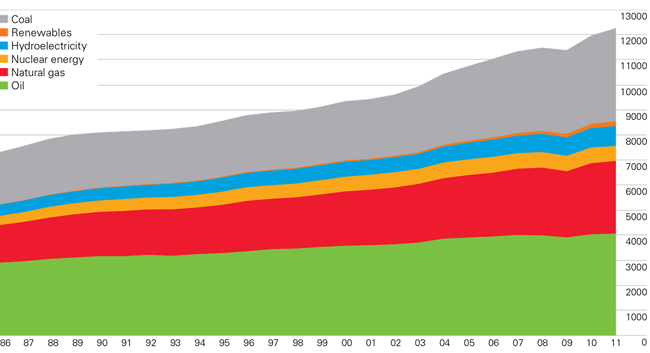
\includegraphics[scale=0.6]{world_Consumption.jpg}
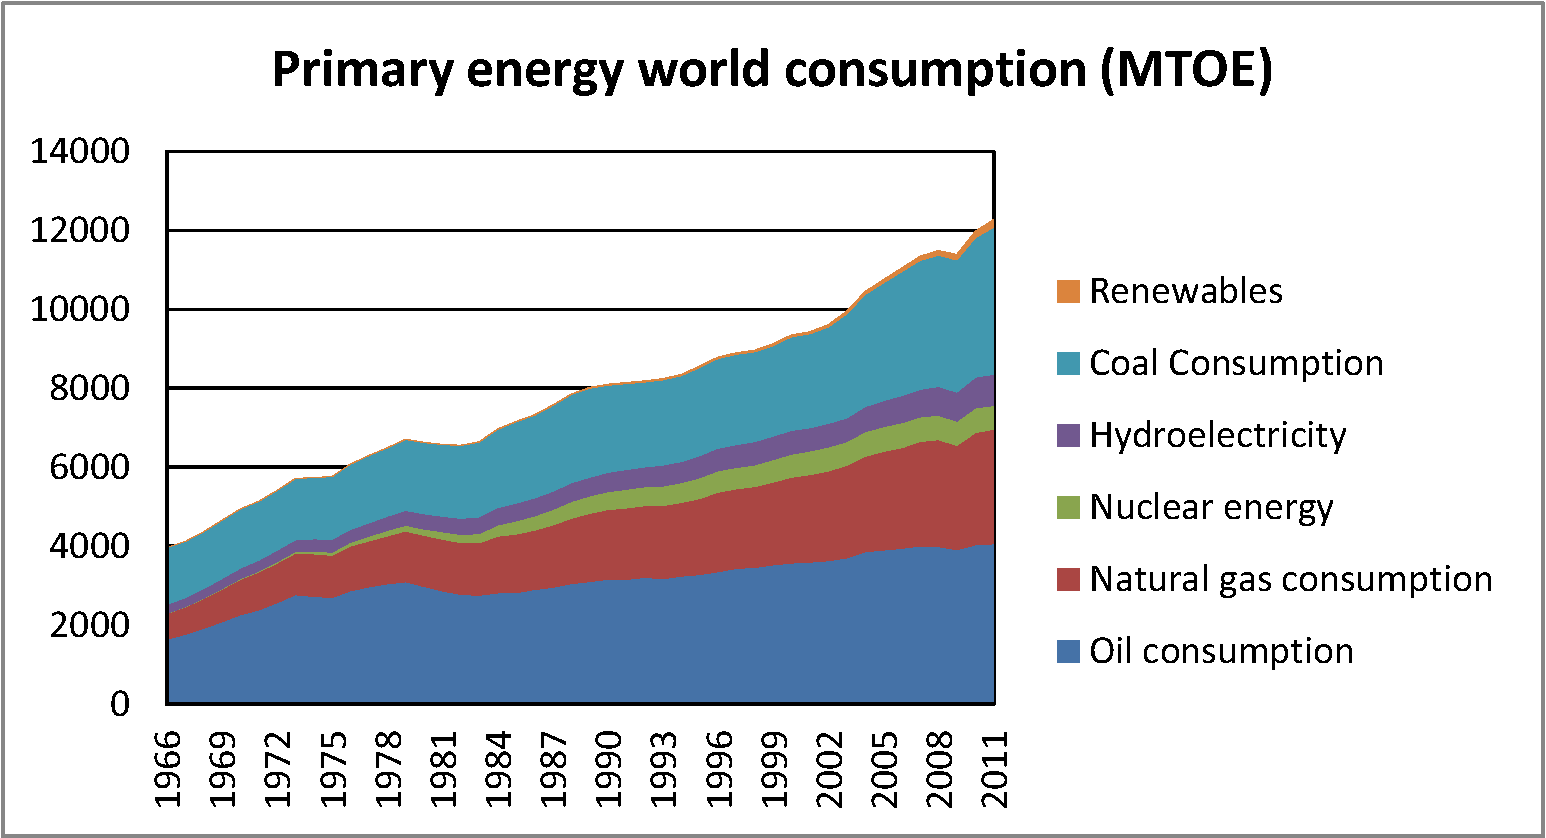
\includegraphics[scale=0.6]{world_Consumption.pdf}
\caption{Figure is from BP statistical review of world energy 2012, METO means million tonnes oil equivalent.}
\label{wpec}
\end{figure}

It is urgent to explore more sustainable and healthy energy sources. From Fig. \ref{wpec}, one will notice that renewable energy (mainly solar energy, wind power, hydropower and 
geothermal energy) in 2012 accounts for around 2\% of energy consumption globally. It is important to focus on the renewable energy research from a long term point of view. The solar energy technology is one of the hot topic amonge the renewable energy research, 
which is the way to produce electricity from the energy of the sun. There are mainly three kinds. The first one is solar thermal, which is mainly
intended to the place where has higher demand for hot water. The second one is solar chemical, which takes advantage of solar energy by absorbing sunlight in a chemical reaction.
The last one is solar photovoltaics (solar cell), which is the way to use solar panels to convert sunlight into electricity. 



In the worldwide, so many reseachers are working on the field of solar cell, so the conversion efficiency in all different types of solar cell is improved remarkably. 
From Fig. \ref{nrel}, one can notice that the highest efficiencies for thin-film technology had exceed 20\% and the maximum efficiency of multijunction cells is over 40\%.
Therefore, the solar cell is a very important and promising way to produce the renewable energy.

\begin{figure}[H]
\centering
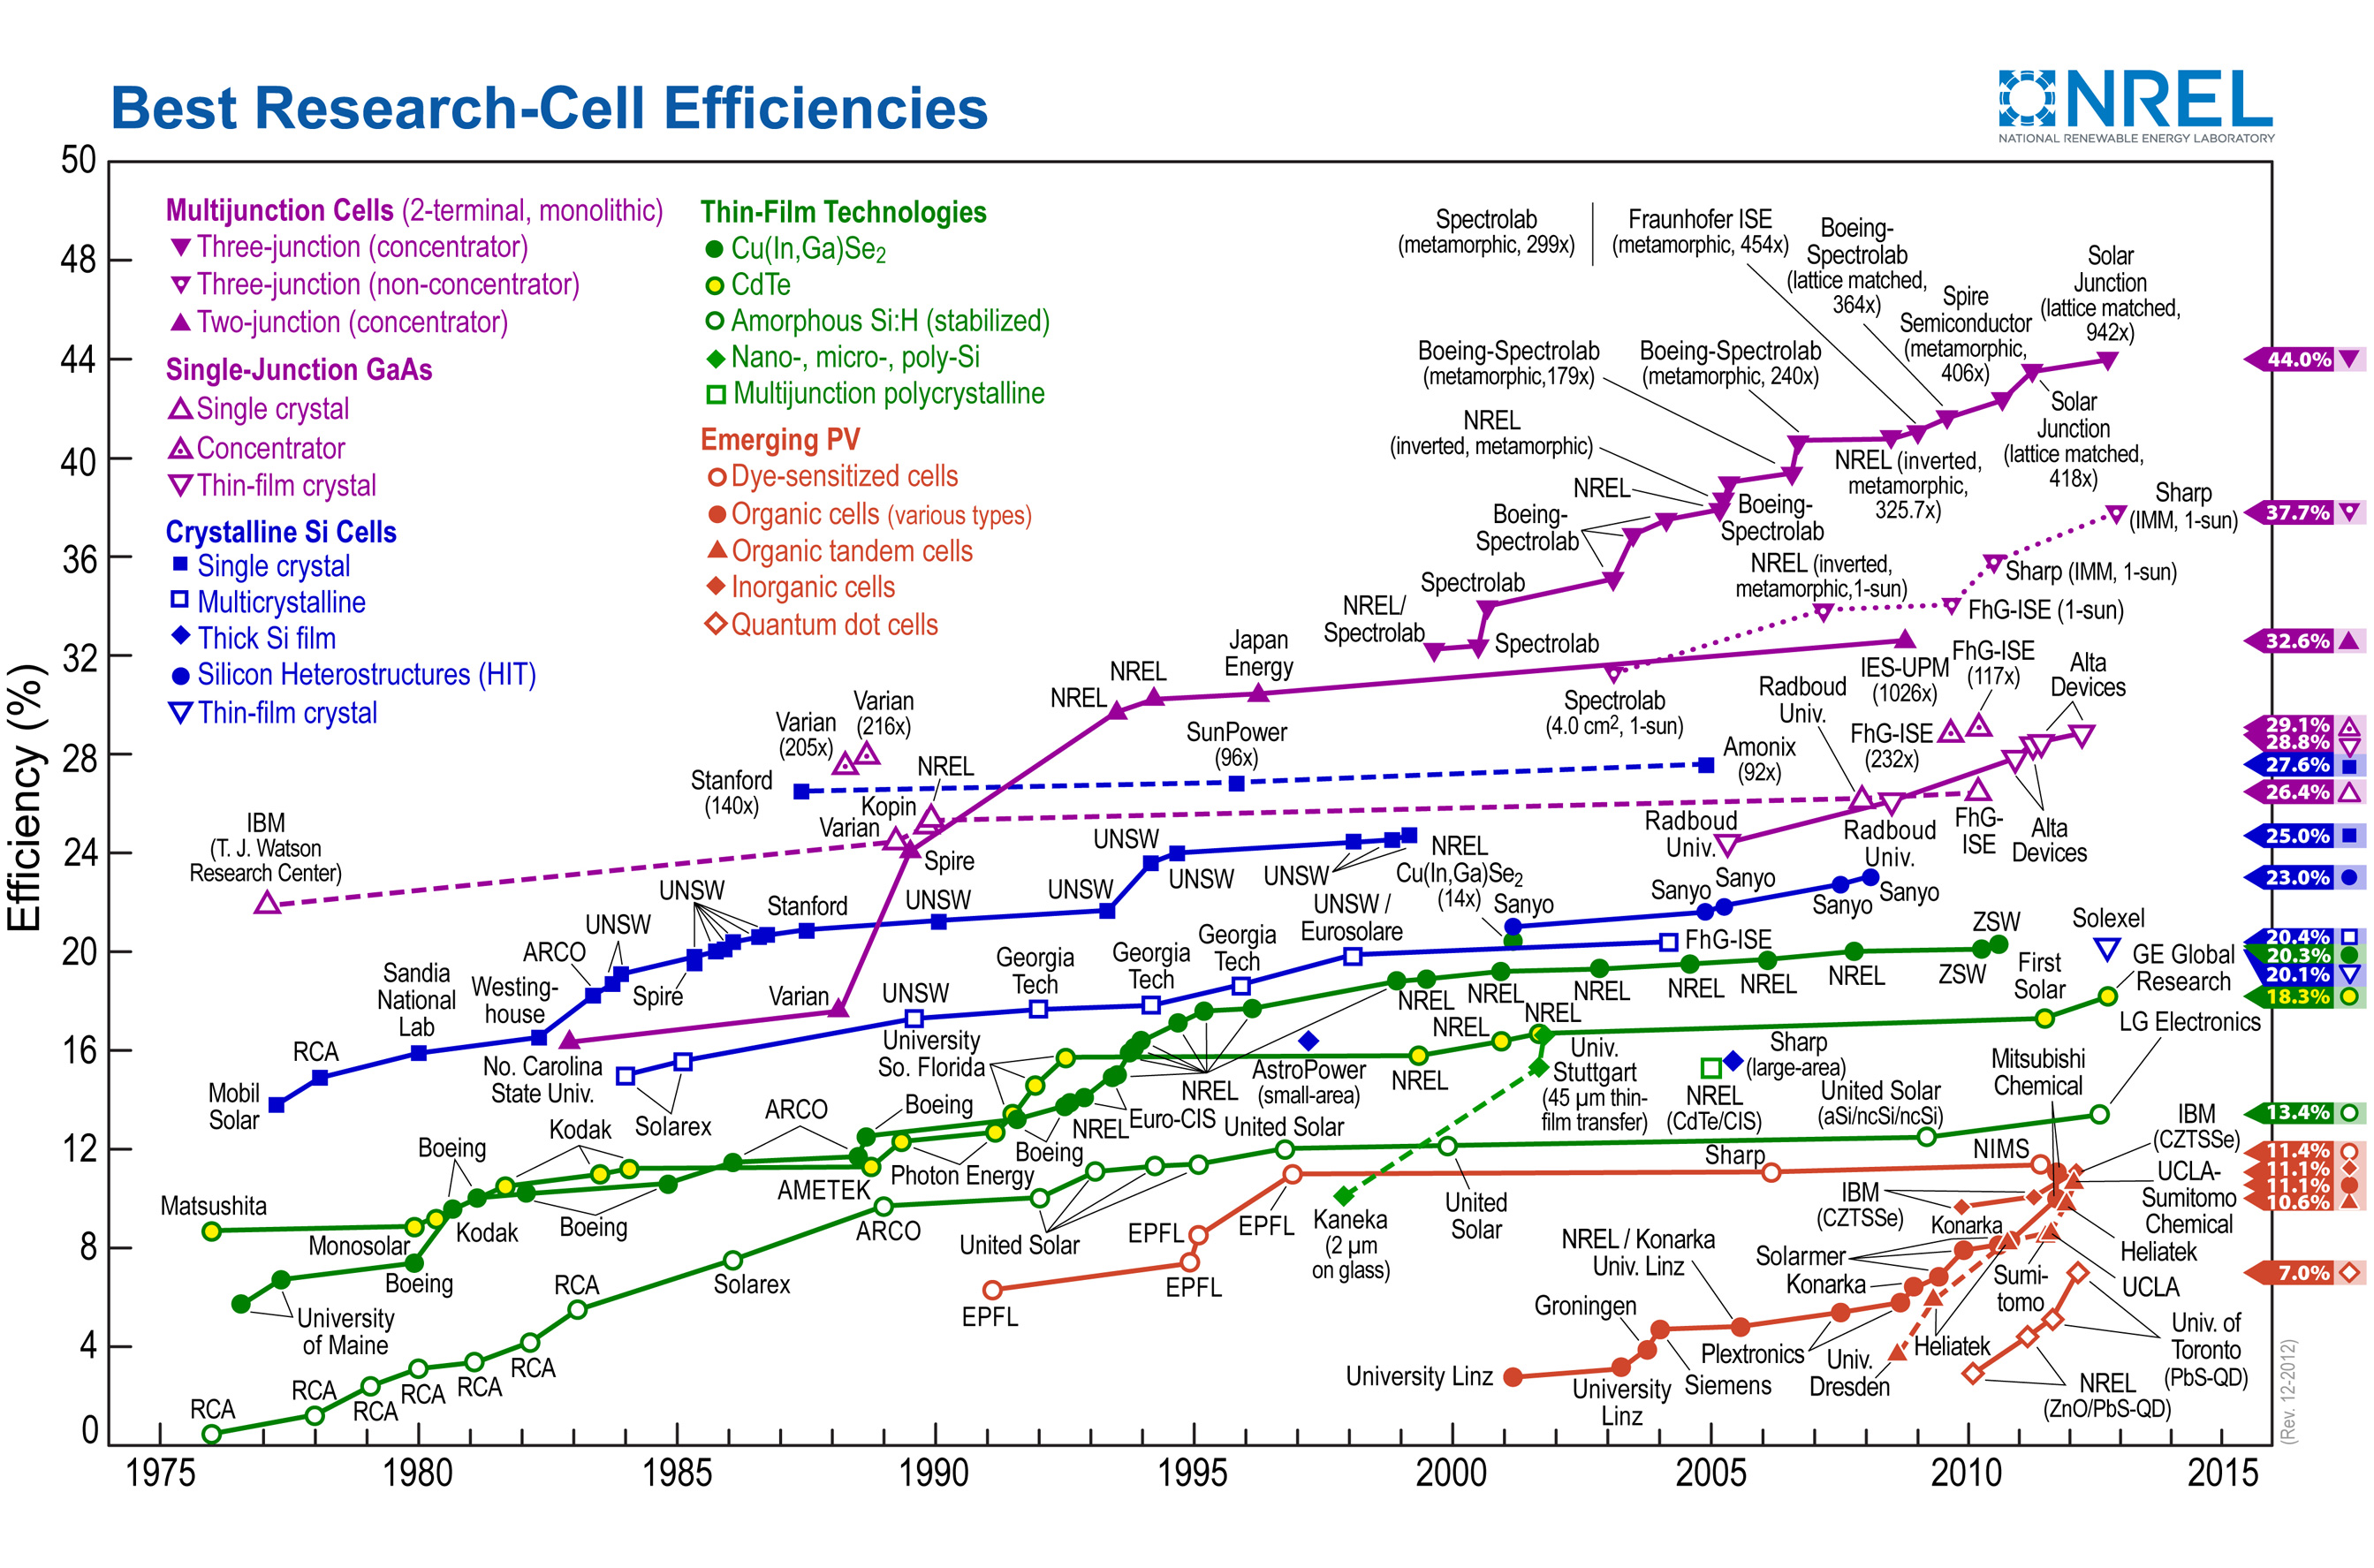
\includegraphics[scale=0.16]{efficiency_chart.jpg}
\caption{Best research-cell efficiencies. Figure is from National Renewable Energy Laboratory (NREL), Golden, Colorado.}
\label{nrel}
\end{figure}


\section{Solar cell materials}
First, a brief history of solar cell is demonstrated. In 1839,  French physicist A. E. Becquerel revealed the photovoltaic effect for the first time, then Charles Fritts built the first solid state photovoltaic (PV) cell using semiconductor selenium in 1883,
it is not until 1941 that the first silicon-based solar cell is demonstrated, until now, there are many different solar cells. The reason why 
better solar cell do not come out yet is that solar cell is expected to not only high efficiency but also environmentally friendly and 
low cost. It means that the process of growth and manufacturing solar cell is cheapter, moveover, it has longer application life, in addition,
the raw material should be abundant and non-toxid.




Currently, there are mainly four kinds of solar cell materials, and they are crystalline silicon (Si) solar cell, thin-film solar cell, dye-sensitized solar cell and organic solar cells.

The solar cell based on silicon dominates the solar world, and more than 90\% of the total PV market is dominated by it.
This kind of solar cell takes advantage of different forms of silicon, that is, monocrystalline silicon, polycrystalline silicon and others. However, silicon is
an indirect band gap material, moreover, the cost is relatively expensive.

 


The thin film solar cells based on some absorber materials, such as the copper indium gallium (di)selenide (CIGS), copper zinc tin sulfide (CZTS) and copper zinc tin
selenide (CZTSe). All of them have direct band gap. The conversion efficiency of CIGS already reached
up to 20.4\% (efficiency in theory 26\%) by the scientist in the Swiss federal laboratories for materials science and technology at the moment, who develop the thin film solar cells on flexible
polymer foils. Compared with CIGS and CZTS(e), even though silicon has been investigated longer and the technology of fabrication is more mature,
CIGS coverages wider range of the solar spectrum and raw material of CZTS(e) is abundant in the earth. However, it is not easy to control the composition of indium and gallium for the CIGS, 
which will effect the conversion efficiency very much, moreover, the indium is rare element in the earth, it will limite the application scale. CZTS is 
a relatively new material, further studies are needed, and the conversion efficiency is reached up to 11.4\% (efficiency in theory 30\%) at the moment in the lab.


The main material properties of CIGS, CZTS and Si are summarized as the following table:

%%%%%%%%%%%%%%%%%%%%%%%%table
\begin{table}[H]
\begin{center}
\begin{tabular}{|c|c|c|c|}
  \hline
  \multicolumn{4}{|c|}{Main properties of CIGS and CZTS} \\
  \hline
   $ $ & CIGS & CZTS & Si\\ \hline
   Absorption coefficient& $10^5$/cm & $10^5$ (CISe)/cm & $10^4$ \\ 
   Band gap& 1.0-1.7 eV & 1.4-1.5 eV & around 1.1 eV  \\ 
   Renewable& In and Ga limitation & Abundant & Abundant   \\ 
   Crystal structure& Chalcopyrites  & Kesterite and Stannite & Diamond cubic\\ 
  \hline
\end{tabular}
\caption{}
\end{center}
\end{table}



The dye-sensitized solar cell and organic solar cells are also promising due to the lower cost. The dye-sensitized solar cell takes advantage of the semiconductor which is formed between a photo-sensitized anode and an electrolyte.
The organic solar cells is a kind of polymer solar cell which uses organic electronics. Both of this two solar cells are not discussed deeply in this licentiate.


\subsection{CIGS cell structure}
The basic and brief introduction of CIGS cell structure is described in the Fig. \ref{cigs_cells}. Glass is used as the substrate and a p-type CIGS absorber layer is placed after 
the Mo deposition (back contact), then a n-type buffer layer (CdS) is covered on the top of the CIGS absorber.
At the last, the buffer layer is overlaid with a ZnO transparent and conductive layer.

\begin{figure}[H]
\centering
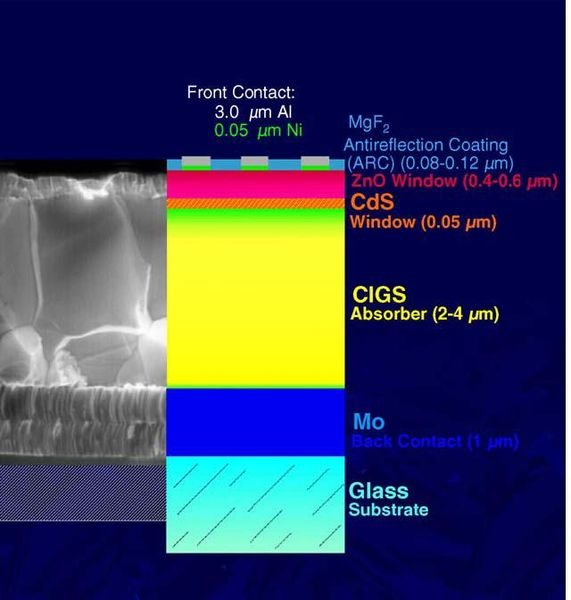
\includegraphics[scale=.5]{CIGS_Structure.JPG}
\caption{CIGS solar cell structure in experiment.}
\label{cigs_cells}
\end{figure}


%{\color{red} ???????????????????????????? here I have to insert figure ?????????????????????????????????}



\subsection{Candidate of solar cell materials}


Potential solar cell materials need to fullfil several properties, such as large absorption coefficient and the band gap range of around 1 to 1.6 eV. Therefore, there 
are quite many materials satisfying the requirement. However, some other properties are needed to be considered as well, such as cost, enviromental safety
and others. Thereby, only some of them is suitable to produce in reality. In the Fig. \ref{lscm}, evolution for several solar cell materials is illustrated. 

\begin{figure}[H]
\centering
%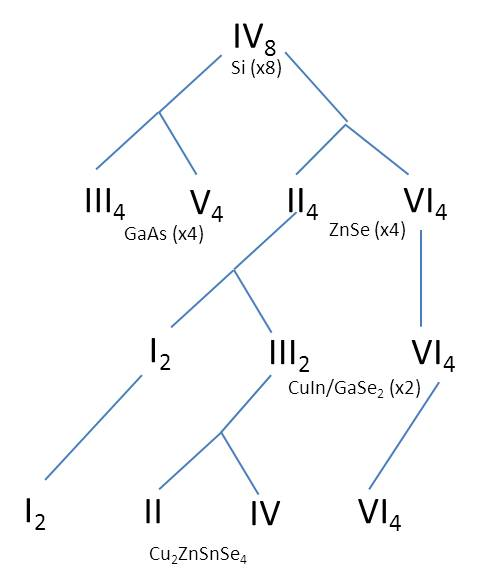
\includegraphics[scale=0.8]{compounds.jpg}
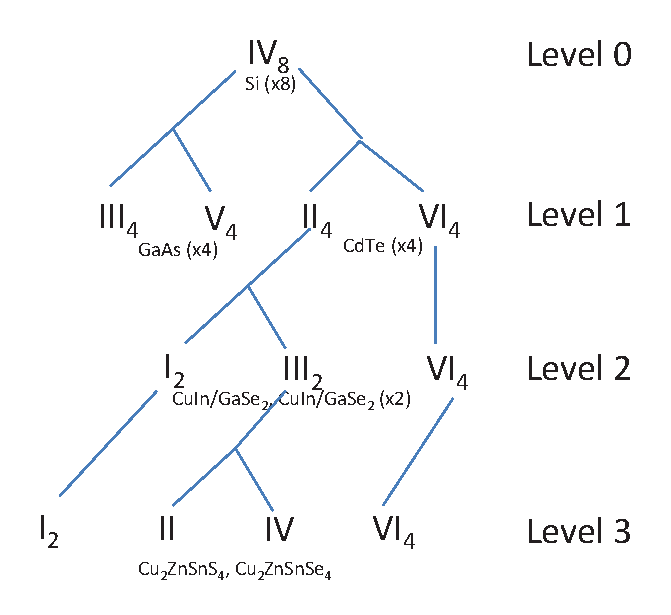
\includegraphics[scale=0.8]{compoundsemicondctor1} 
\caption{Tree of tetragonal bonded semiconductor, the roman numerals means the group numbers in the chemical element periodic table, the subscript means the number of elements.}
\label{lscm}
\end{figure}


From above Fig. \ref{lscm}, based on group number IV element silicion (level 0) in the chemistry element periodic table, two categories semiconductor materials are deduced (level 1), such as gallium arsenide (GaAs) in group III-V and cadmium telluride (CdTe)
in group II-VI. The element in group II in level 1 could be further divided into elements in group I and III, such as CIGS and CIGSe (level 2). From the group III in level 2, the element is possible to
be substituted from group II and IV in level 3, such as CZTS and CZTSe.



\section{Basic pricinple of semiconductor}

The radiation from sun seperates electron-hole pairs in semiconductor, therefore, the electrons and holes are flowing in two different directions due to 
the voltage formed by p-n junction. The load is working properly if it is connected with the semiconduction device. The basic pricinple of semicondctor
will be demonstrated in this section, and the semiconductor silicon is choosen as an example. 

\subsection{Sunlight}
Sunlight is a portion of the radiation by the sun, like infrared, visible, and ultraviolet light.
The spectrum of the sun is more or less a black body with a temperature of about 6000 K (Fig. \ref{spectrumsun}). 



\begin{figure}[H]
\centering
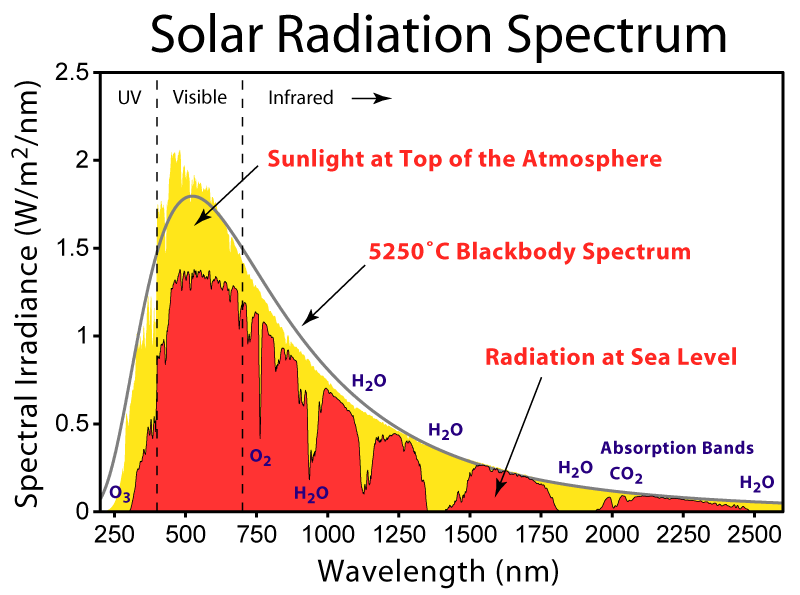
\includegraphics[scale=.32]{spectrumsun.png}
\caption{Solar irradiance spectrum.}
\label{spectrumsun}
\end{figure}

The sunlight is transported by particles, named photons. The optical band gap in semiconductor is related with the photons. In Fig.\ref{maxgap}, the Shockley–Queisser limit presents 
the maximum possible efficiency of a single junction solar cell under un-concentrated sunlight. Therefore, if the band gap is too high, the photons can not be absorbed and 
the efficiency of solar cell is lower. Conversely, if the band gap is too low, the photons carry too much energy. It generates a lot of electrons, most of the energy is lost in the form of heat, therefore, the efficiency of
solar cell is lower as well. 
 

\begin{figure}[H]
\centering
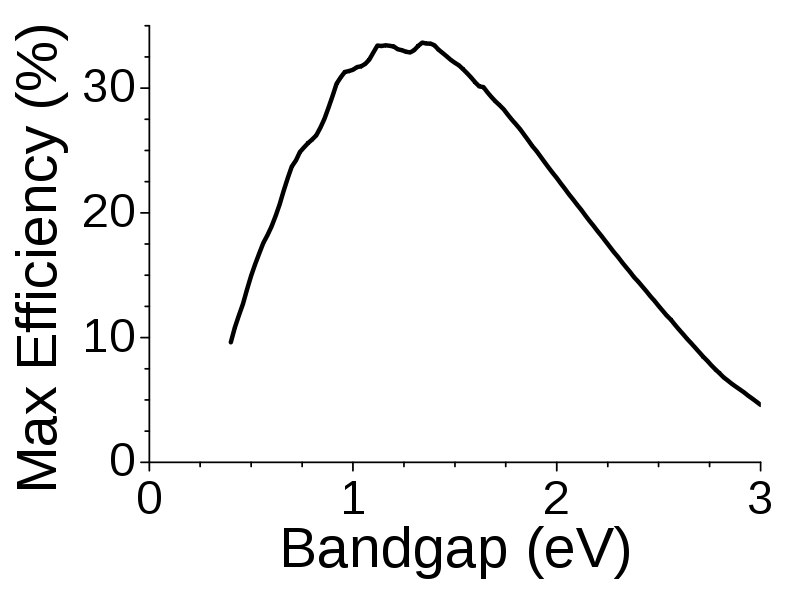
\includegraphics[scale=.25]{maxgap.png}
\caption{The maximum possible efficiency of a single junction solar cell.}
\label{maxgap}
\end{figure}

\subsection{Silicon} 
The single silicon atom has 14 electrons, but only 4 valence electrons can participate in the formation of a chemical bond. In Fig \ref{singleatom}, the dot with while color denotes the empty states, 
the dot with other colors denotes the electrons. $n1$, $n2$ and $n3$ means the electron shell. The dashed line means the effective potential.

\begin{figure}[H]
\centering
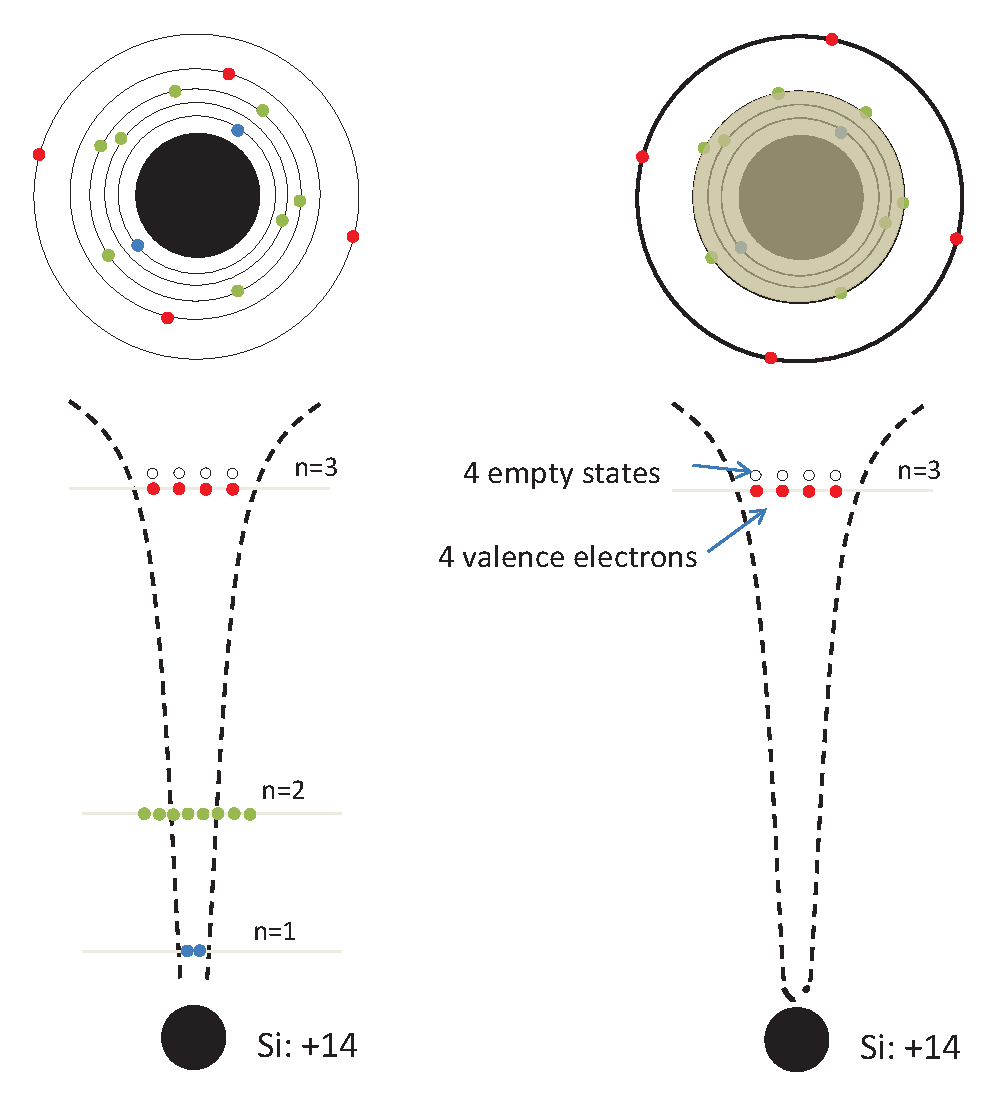
\includegraphics[scale=.45]{singleatom}
\caption{Single silicon atom. Left panel: the full electron configuration for single silicon atom. Right panel: the simplified of left panel, only 4 valance electrons are considered.}
\label{singleatom}
\end{figure}

Fig. \ref{crystal} is the 2D version of silicon crystal.
The silicon has four bonds for each silicon atom to form crystal (four overlap regions for each silicon atom). Silicon atoms form covalent bonds, and each covalent bond
has two electrons (one of the four overlap regions).
 


\begin{figure}[H]
\centering
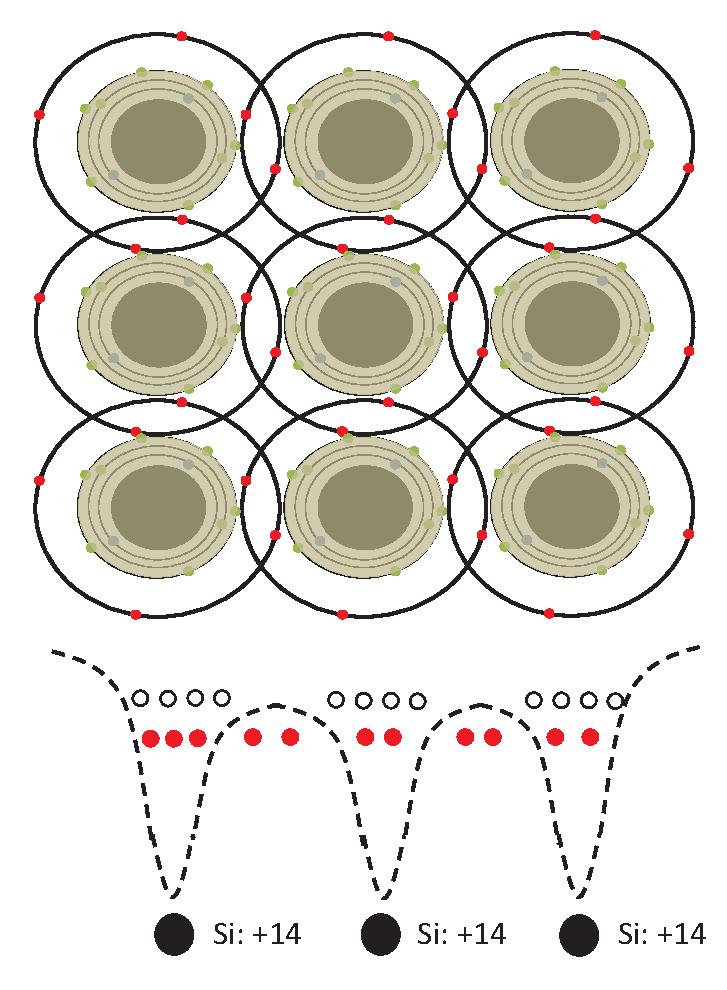
\includegraphics[scale=.6]{crystal}
\caption{Silicon crystal. Each silicon atom shares of pairs of electrons (red dots in the overlap regions) with neighbour atoms.}
\label{crystal}
\end{figure}


From Fig. \ref{combination}, if the sunlight is acrossing this crystal silicon, the electrons which are in valence bands has the possiblities to jump to conduction bands across the band gap.
There are some positive (negative) "holes" (electrons) left in the valence (conduction) bands (left panel in Fig. \ref{combination}). The paired electron-"hole" will recombination if there is no external 
"force" seperating them (right panel in Fig. \ref{combination}).


\begin{figure}[H]
\centering
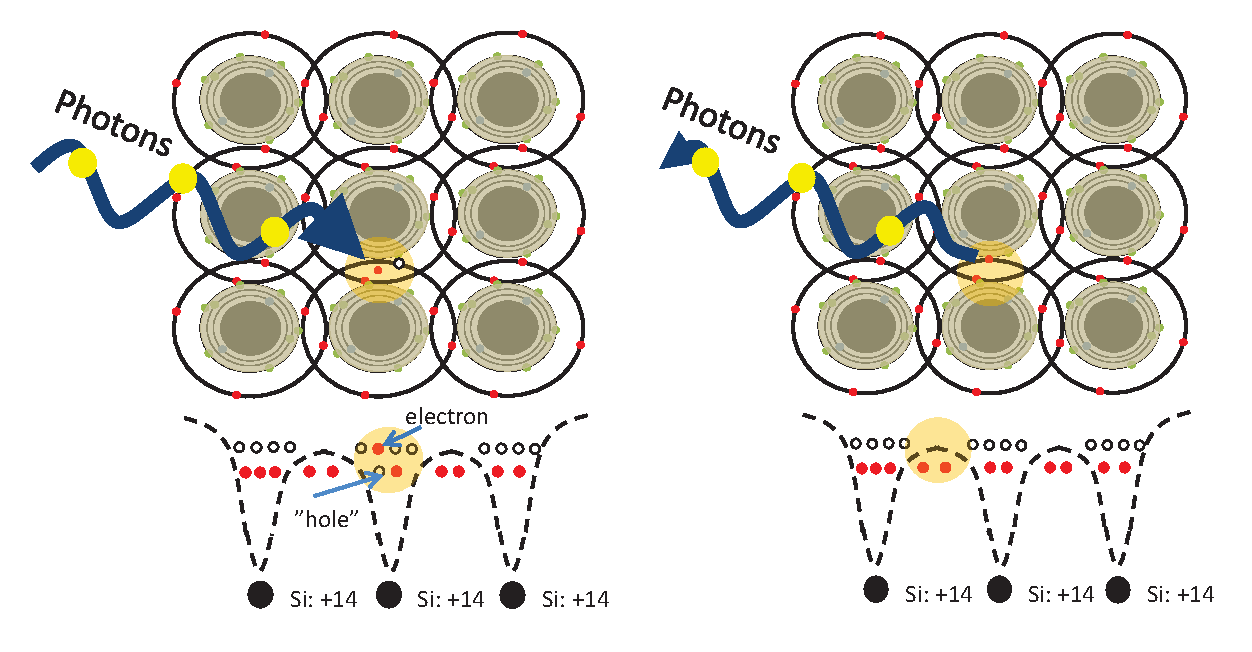
\includegraphics[scale=.6]{combination}
\caption{Left panel: the electrons absorpting photons in valence band are excited to conduction bands. Right panel: the electrons in conduction bands jump back to 
valence bands while emitting photons.}
\label{combination}
\end{figure}


\subsection{p-n junction}

In order to seperate the paired hole-electron and avoid of recombination, doping is needed inside the material silicon. 

If one of the silicon atom is 
substituted by one phosphorous (P) atom, which has 5 valence electrons. Therefore, there is one more extra electron left (left panel in Fig. \ref{nptypes1}). Because there is 
one negative charge exsiting in this semiconductor, therefore, this kind of semiconductor is called n-type doping semiconductor (n means negative). 
If one silicon atom is substituted by one boron (B) atom, which has 3 valence electrons. Therefore, the corresponding covalence bond is not formed
properly, that is, one valence electron is missed (right panel in Fig. \ref{nptypes1}). The boron atom is called acceptor since it has the ability to accept one more electron. Because 
there is one postive charge (hole) in this semiconductor, thereby, this kind of semiconductor is called p-type doping semiconductor (p means positive). 

\begin{figure}[H]
\centering
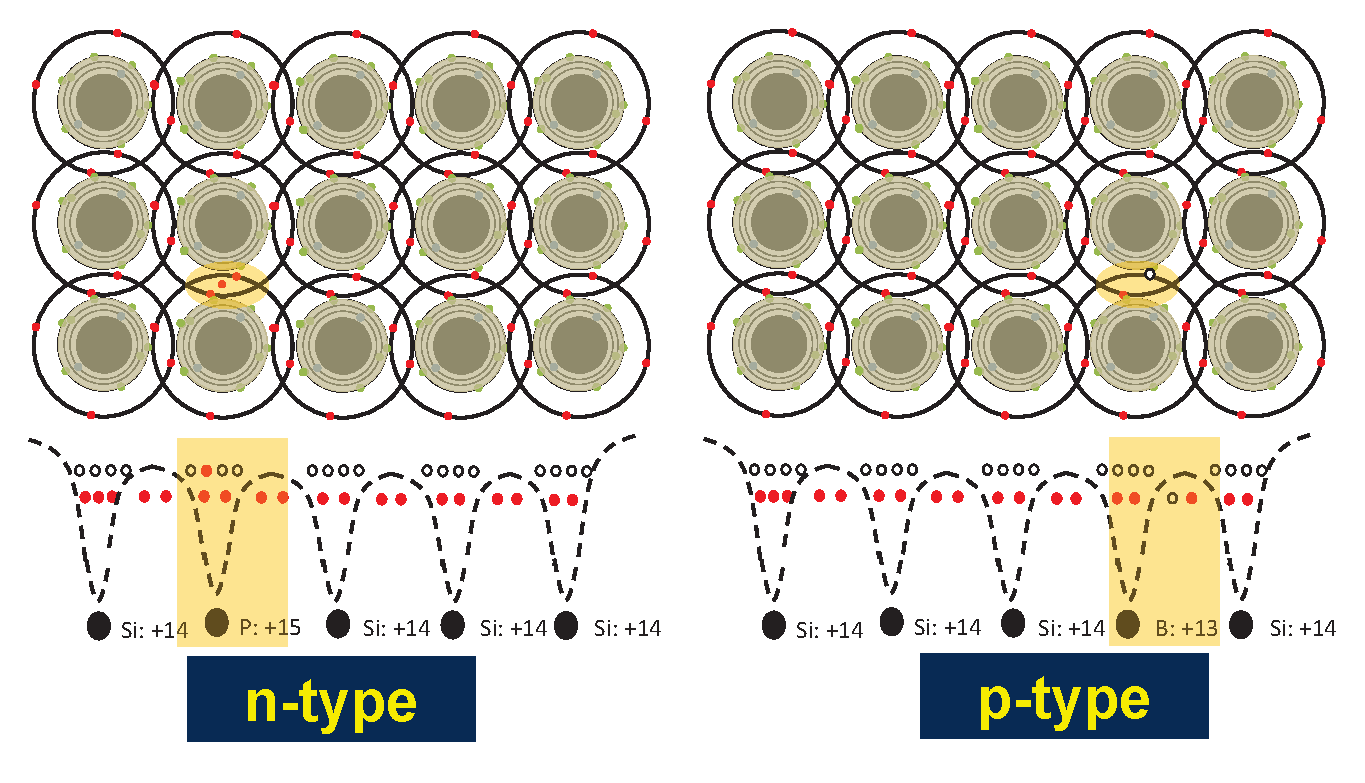
\includegraphics[scale=.6]{nptypes1}
\caption{Left panel: n-type semiconductor. Right panel: p-type semiconductor.}
\label{nptypes1}
\end{figure}



If the p-type and n-type semiconductor are somehow put together, thereby, p-n junction is formed (Fig. \ref{nptype2}). Inside the p-n junction, the extra electron and "hole" is prone to
be paired. Therefore, there is an internal electric field formed (right panel in Fig. \ref{nptype2}). The direction of field is from n-side to p-side. 

\begin{figure}[H]
\centering
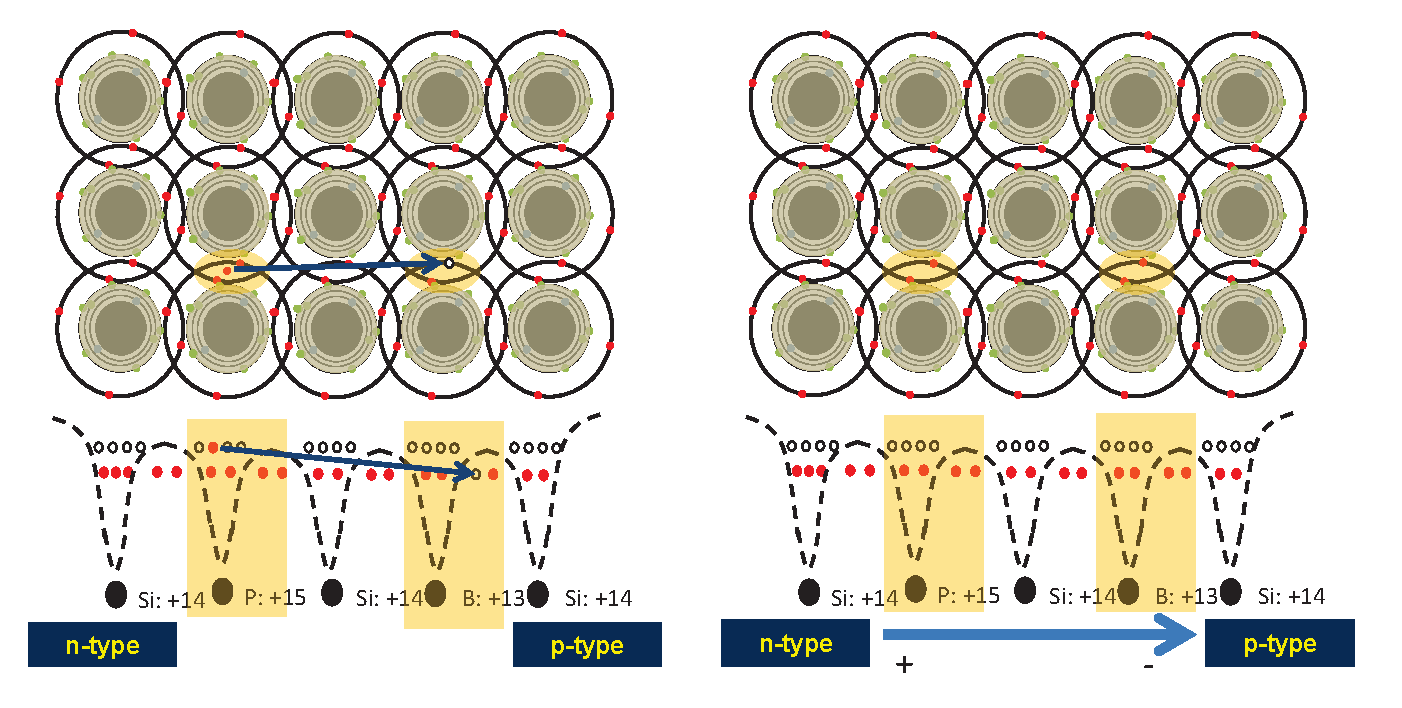
\includegraphics[scale=.6]{nptype2}
\caption{Left panel: the electron-hole is prone to be paired. Right panel: the internal electric field is formed due to the doping.}
\label{nptype2}
\end{figure}


The electrons and holes will move to different direction due to the internal electric field when the sunlight across to this p-n junction.

\begin{figure}[H]
\centering
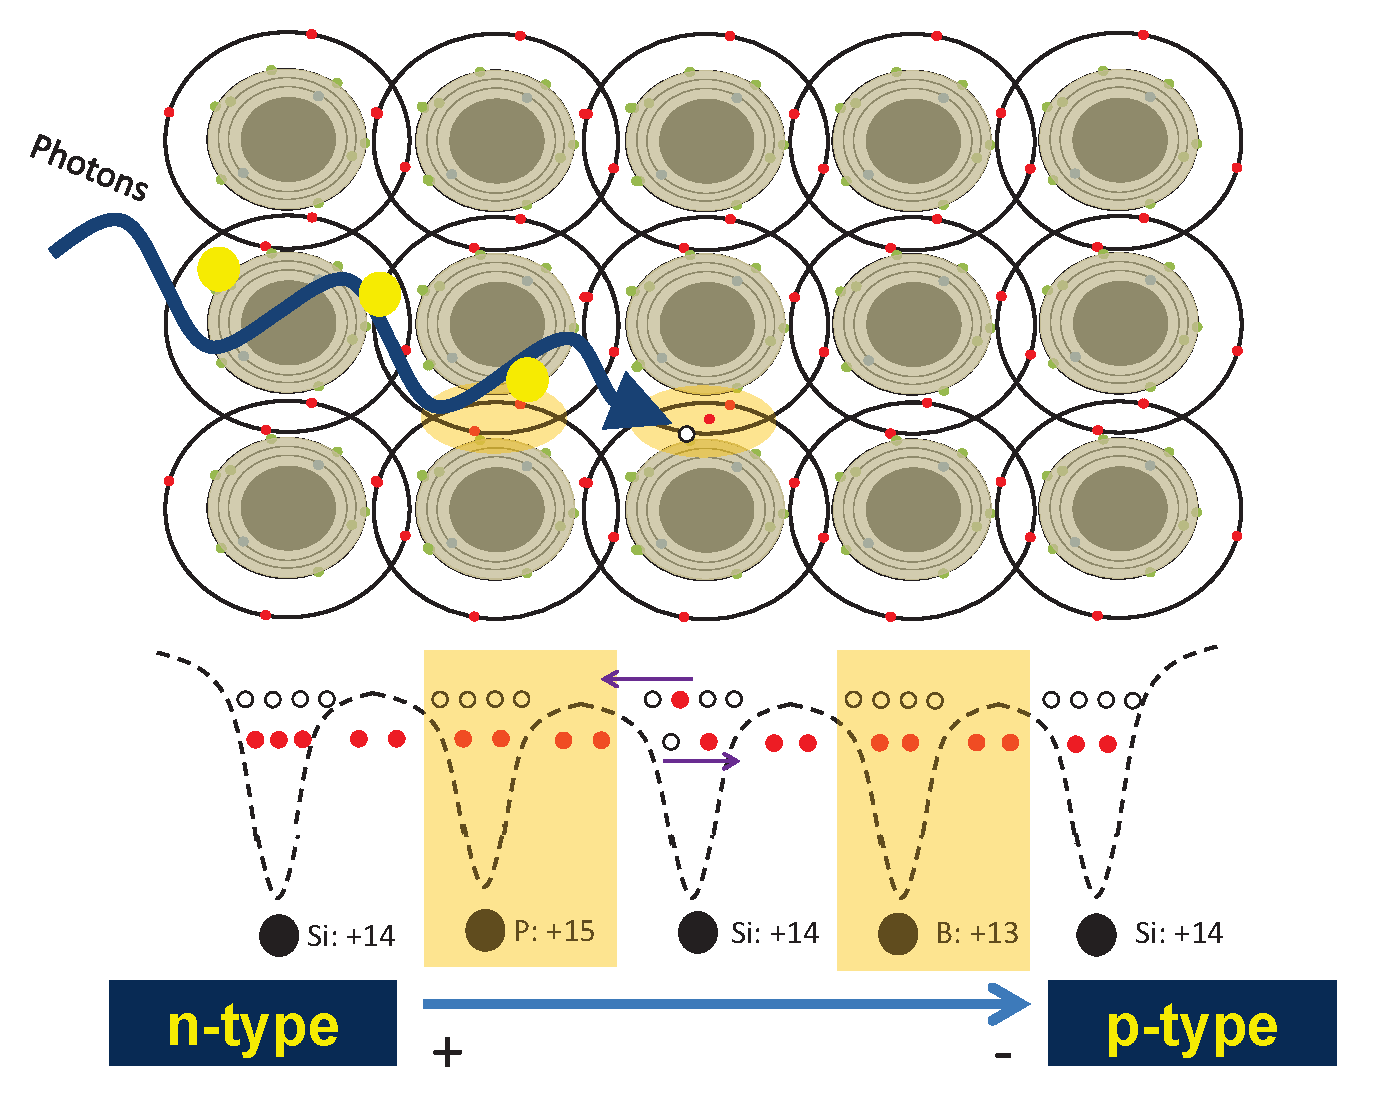
\includegraphics[scale=.4]{scr1}
\caption{The electrons and holes are moving to oppsite direction, the puple line in the middle indicates the movement direction.}
\label{scr1}
\end{figure}


It is also possible to demonstate the p-n junction in terms of band structure. First, the concept of Fermi level, valence band and conduction band is needed to be understood.
In solid, the band structure is formed due to huge amount of atoms which interact each other. The electron in solid occupy the energy levels from lowest state to some
energy state. Therefore, this energy where all states below are occupied and all above are empty is called Fermi level. At absolute zero temperature, the valence band (VB) is the highest range of energy level which
is occupied. After VB, the band is named conduction band (CB).

In Fig.\ref{scr136}, the "holes" will move to the p-type semiconductor if they arrive at the space charge region (SCR). The electrons will move to the n-type semiconductor if they reach to the SCR.


\begin{figure}[H]
\centering
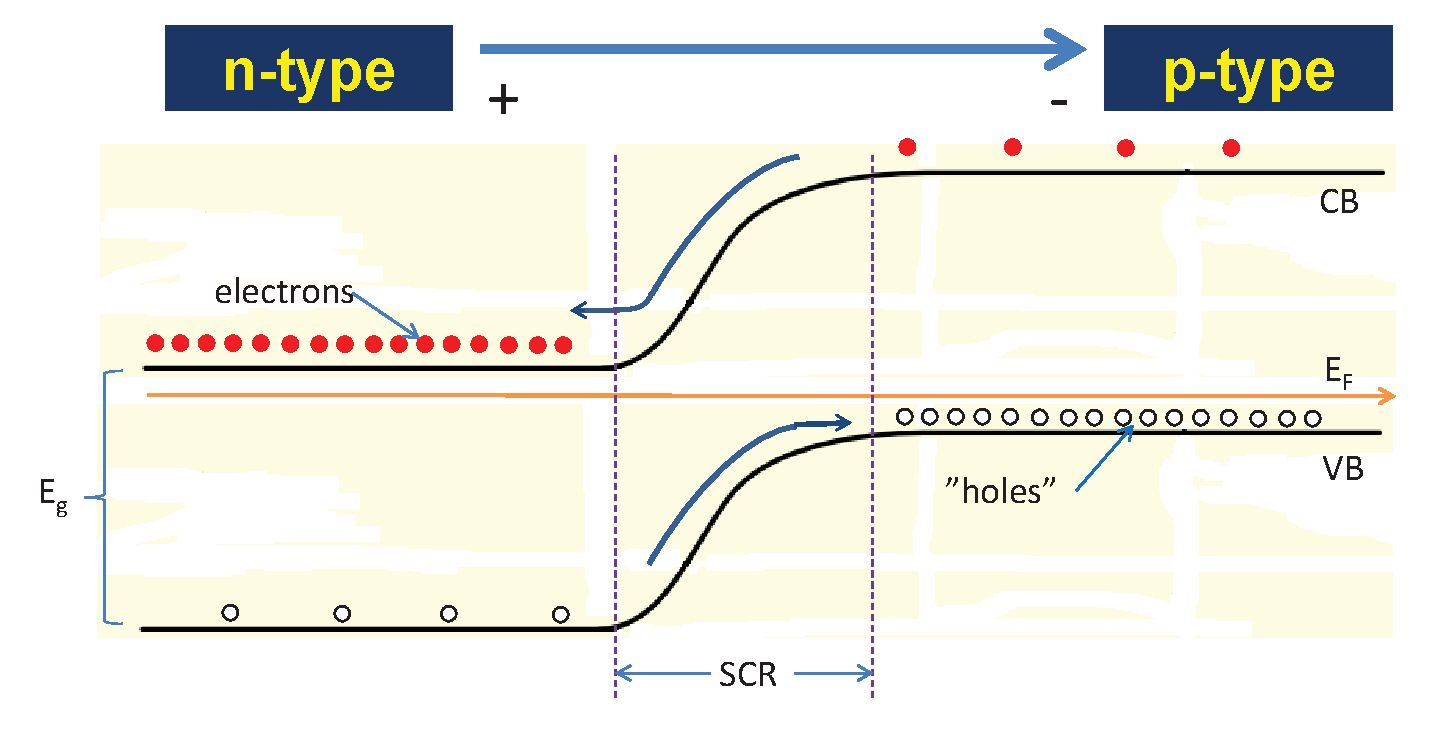
\includegraphics[scale=.5]{scr2}
\caption{Band-bending at the p-n junction. $E_g$ is the band gap and $E_F$ is the Fermi level, SCR denotes space charge region.}
\label{scr136}
\end{figure}

Therefore, the load will work properly if the solar cell based on the p-n junction is assembled in a closed loop.

\section{Summary}
In this licentiate, the main research material is CIGS, the motivation is that CIGS is a very promising thin film absorber material, although the macroscopic 
properties of CIGS already are fairly well understood, there are only little research about the details of the electronic energy band dispersion near the uppermost
VBs and CB, which is important for analyzing and understanding electrical properties. 

There are two major issues discussed, the first one is that the parameterization of the energy bands for the three uppermost VBs and the lowest CB is presented, and compared with results from the parabolic band approximation and non-parablic band
dispersion. Another one is that since the low temperature SE study of CIGS at the temperature of 40 K is rare, the ${\varepsilon}$ spectra of CIGS is compared and analysed by experiment and theoretical
calculation. 


\chapter{Electronic structure calculations }
\label{ch:dft}

\section{The quantum many-body problem}
\label{ch:mb}

\noindent A solid material contains a huge number of atoms (around $10^{23}/cm^3$), and the atom is constructed by nuclei and electrons. 
According to the quantum mechanics principles, all the properties of any system are known if one can figure out a way to solve 
the quantum many-body Schrödinger equation exactly. Let us start from the time-independent many-body Schrödinger equation,

 
\begin{equation}\label{ssth}
 {\hath} {\wf} = {E} {\wf},
\end{equation}

\noindent where $\wf$  is the exact wavefunction for the above Schrödinger equation, $\textbf{r}_\textit{i}$ and $\textbf{R}_\textit{I}$  stands for electron and
nucleus coordinators, respectively.

In the Eq. (\ref{ssth}), $E$ is the total energy of the system, and $\hath$ is the Hamiltonian which has the following form:

\begin{equation}\label{th}
\begin{split}
& \hath = - \sumi<i> {\frac{\hbar^{2}}{2 m_{\textit e}}}   \nablaia<i> - \sumi<I> {\frac{\hbar^{2}}{2 M_\textit{I}}} \nablaia<I>  - \sumij<i><I> \frac{Z_\textit{I}\ e^2}{4 \pi \varepsilon_0 |\textbf{r}_\textit{i}-\textbf{R}_\textit{I}|} \\
& + \frac{1}{2} \suminj<i><j> \frac{ e^2}{4 \pi \varepsilon_0 |\textbf{r}_\textit{i}-\textbf{r}_\textit{j}|} + \frac{1}{2} \suminj<I><J> \frac{Z_\textit{I} Z_\textit{J}\  e^2}{4 \pi \varepsilon_0 |\textbf{R}_\textit{I}-\textbf{R}_\textit{J}|},
\end{split}
\end{equation}


\noindent where the indices $\textit{i}$, $\textit{j}$ are used for electron and $\textit{I}$, $\textit{J}$ are used for atomic nuclei, $Z_\textit{I}$ means the charge of the $\textit{I}$-th nucleus,
$\textit{M}$ denotes the nuclear mass, $m_e$ is the electron mass, $\varepsilon_0$ is vacuum permittivity.

In atomic units, the reduced Planck constant $\hbar$, the electron mass $m$, the Bohr radius $a_0$, and the electron charge
$e$ are equal to 1. The Bohr radius is given by the formula $a_0$ = ${\hbar} / {(mc\alpha)}$, where $\alpha$ is the fine structure
constant ($\alpha$ = ${e^2}/{(4 \pi \varepsilon_0 c \hbar)}$) , so the velocity of light in atomic units is $c$ = $1/{\alpha}$ and ${e^2}/{(4 \pi \varepsilon_0)}$= 1. The Schrödinger Eq. (\ref{th}) in atomic units has 
the following form:

\begin{equation}\label{sth}\begin{split}
&\hath = - \sumi<i>   \frac{{{\nabla}_{\textit{i}}^{2}}}{2} - \sumi<I> \frac{{{\nabla}_{\textit{I}}^{2}}}{2 M_\textit{I}}  - \sumij<i><I> \frac{Z_\textit{I}}{|\textbf{r}_\textit{i}-\textbf{R}_\textit{I}|} \\
& + \frac{1}{2} \suminj<i><j> \frac{1}{ |\textbf{r}_\textit{i}-\textbf{r}_\textit{j}|} + \frac{1}{2} \suminj<I><J> \frac{Z_\textit{I} Z_\textit{J}\ }{|\textbf{R}_\textit{I}-\textbf{R}_\textit{J}|}.
\end{split}\end{equation}


\noindent In Eq. (\ref{sth}), the first and second terms are the kinetic energy operator of the electron and nuclei, respectively.
The other terms in order are Coulomb interactions between electrons and nuclei, electrons and electrons and nuclei and nuclei.

\noindent Since there are so many atoms to calculate in reality, more importantly, the exactly form of the wavefunction is unknown,
so one can not solve the Eq. (\ref{ssth}) exactly at present. To approximate the exact solution, 
generally one can divide it into three different levels, the first level is the Born-Oppenheimer approximation and the second level is Hartree,
Hartree-Fock (HF), density functional theory (DFT) and Kohn-Sham (KS) equation, and the last level is to solve the secular equation, 
which is an equation that is solved to find the eigenvalue of matrix.

\section{The Born-Oppenheimer approximation}
\label{ch:boa}

\noindent In order to simplify the Eq.  (\ref{ssth}), the first attempt is to seperate the wavefunction of electrons and nuclei, but since there is a couple term between the electron and nucleus in the Schrödinger Hamitonian in Eq. (\ref{sth}), 
thereby one can not do that simply. On the other hand, let us observe the Eq. (\ref{sth}) again, there exists a small value ${1}/{M_I}$, which is part of the nucleus kinetic energy
operator term, the reason is that the mass of nucleus is much larger than that of electron, so the nuclei are treated as fixed. The result is that the electrons is seen as interacting under both the external potential caused by nuclei that are fixed in 
some positions and that of the other electrons. A more vividly description is seen from Fig. \ref{figbo}:
%figure
\begin{figure}[H]
\centering
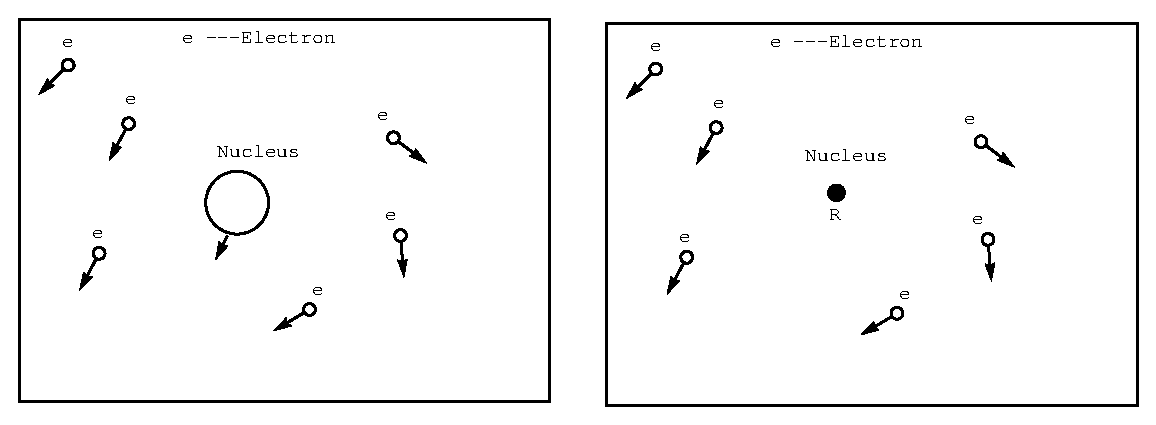
\includegraphics[scale=.7]{system.eps}
\caption{Left panel: normal interacting system. Right panel: the Born-Oppenheimer approximation. The arrows denotes the movement of the nucleus or electron.}
\label{figbo}
\end{figure}

\noindent The separation of motion between electrons and nuclei is called the Born-Oppenheimer approximation, since the position of nuclei is fixed, one can define:

\begin{equation}\label{nwf}
{\wf}  {\approx}  {\Psi_{ \textit{BO}} ( \{ {\textbf{r}_{\textit{i}}},\textbf{R}_{\textit I} \}) } = {\theta(\{{\textbf R}_{\textit I}\})} {\Psi'(\{\textbf{r}_{\textit i}\}; \{{\textbf R}_{\textit I}\})},
\end{equation}


 \noindent where ${\Psi'(\{\textbf{r}_{\textit i}\}; \{{\textbf R}_{\textit I}\})}$  is the electrons wavefunction in the Born-Oppenheimer approximation, the semicolon means that $\textbf R_I$ is only discrete value belonging to the set of atomic positions. 
 
The Eq. (\ref{sth}) can be defined as:

\begin{equation}\label{nh}
 {\hath} = - \sumi<I> \frac{{{\nabla}_{\textit{I}}^{2}}}{2 M_\textit{I}} + {\hath}_{BO}.
\end{equation}

where 

\begin{equation}\label{both}\begin{split}
&{\hath}_\textit{BO}\ =\ - \sumi<i>   \frac{{{\nabla}_{\textit{i}}^{2}}}{2}  - \sumi<i> V_{ext}(\textbf{r}_{\textit{i}})  + \frac{1}{2} \suminj<i><j> \frac{1}{ |\textbf{r}_\textit{i}-\textbf{r}_\textit{j}|} + \frac{1}{2} \suminj<I><J> \frac{Z_\textit{I} Z_\textit{J}\ }{|\textbf{R}_\textit{I}-\textbf{R}_\textit{J}|} \\
&\ = \ \hat{T} \ + \ \hat{V}_{ext} \ + \ \hat{V}_\textit{int}\ + \ N_\textit{II},
\end{split}\end{equation}

and

\begin{equation}\label{vext}
V_{ext}(\textbf{r}_{\textit{i}}) =  \sumi<I> \frac{Z_\textit{I}}{|\textbf{r}_\textit{i}-\textbf{R}_\textit{I}|},
\end{equation}

\noindent where ${\hath}_\textit{BO}$  is the Hamitonian for the electrons within the Born-Oppenheimer approximation. The subscript $ext$ means $external$ in Eq. (\ref{vext}), this term describes the external potentials interaction. 

\noindent Thereby, the new Schrödinger equation with Eq. (\ref{nwf}) and Eq. (\ref{nh}) is 

\begin{equation}
 (- \sumi<I> \frac{{{\nabla}_{\textit{I}}^{2}}}{2 M_\textit{I}} + {\hath}_{BO} ) ({\theta(\{{\textbf R}_{\textit I}\})} {\Psi'(\{\textbf{r}_{\textit i}\}; \{{\textbf R}_{\textit I}\})}) = E_{m}(\{{\textbf R_I}\}) ({\theta(\{{\textbf R}_{\textit I}\})} {\Psi'(\{\textbf{r}_{\textit i}\}; \{{\textbf R}_{\textit I}\})}).
\end{equation}
 
\noindent Here, $E_{m}(\{{\textbf R_I}\})$ is the total energy, after some steps of derivation, one can end up with the Eq. (\ref{bose}) :

\begin{equation}\label{bose}
{\hath}_{BO} {\Psi'(\{\textbf{r}_{\textit i}\}; \{{\textbf R}_{\textit I}\})} = E_\textit{BO}{(\{\textbf{R}_{\textit I}\})} {\Psi'(\{\textbf{r}_{\textit i}\}; \{{\textbf R}_{\textit I}\})},
\end{equation}

\noindent where $E_\textit{BO}{(\{\textbf{R}_{\textit I}\})}$ is the energy of this electronic system,

\begin{equation}\label{ise}
( \hat{H}_{I1}+\hat{H}_{I2}+\hat{H}_{I3}+E_{BO}(\{{\textbf R}_{\textit I}\}) ) {\theta(\{\textbf{R}_{\textit I}\})} = E_{m}(\{{\textbf R_I}\}) {\theta(\{\textbf{R}_{\textit I}\})},
\end{equation}

\noindent where

\begin{equation}\begin{split}
 &  \hat{H}_{I1} = - \sumi<I> \frac{{{\nabla}_{\textit{I}}^{2}}}{2 M_\textit{I}}   \\
 &  \hat{H}_{I2} = - \sumi<I> \frac{1}{M_\textit{I}} {\int {\Psi'(\{\textbf{r}_{\textit{i}}\}; \{\textbf{R}_{\textit I}\})}^{\ast} {{\nabla}_{\textit{I}}} {{\Psi'(\{\textbf{r}_{\textit{i}} \}; \{\textbf{R}_{\textit I}\})}} d {\textbf r }} {{\nabla}_{\textit{I}}}  \\
 &  \hat{H}_{I3} = - \sumi<I> \frac{1}{M_\textit{I}} {\int {{\Psi'(\{\textbf{r}_{\textit{i}}\}; \{\textbf{R}_{\textit I}\})}}^{\ast} {{\nabla}_{\textit{I}}^{2}} {{\Psi'(\{\textbf{r}_{\textit{i}} \}; \{\textbf{R}_{\textit I}\})}} d {\textbf r }}. 
\end{split}\end{equation}

\noindent From Eq. \ref{ise}, one observes that the lattice dynamical properties of certain system within the Born-Oppenheimer approximation could be obtained. To solve this equation,
the ground state energy $E_{BO}(\{{{\textbf R}_{\textit I}}\})$ of electron system is needed. Here $\{{\textbf R}_{\textit I}\}$ are the parametrilized values from the atom position.
 

\noindent In summary, the Schrödinger equation of electron and nucleus is derived seperately within the Born-Oppenheimer approximation. When one refers to calculations of the ground state properties,
which means to take use of the Schrödinger equation of electron only, e.g., Eq. \ref{bose}, and Schrödinger equation of nucleus is used for the calculation of lattice dynamics.

One notices that the Eq. \ref{both} is much simpler than Eq. \ref{sth}, but still the equation is not solvable. Further approximations  are needed
to solve this many-body problem.


\section{Hartree, Hartree-Fock approximation and density functional theory}

%\subsection{Hartree and Hartree-Fock approximation}
\noindent From last section, the seperation of wavefunction is given within Born-Oppenheimer approximation, the quantum many-body Schrödinger problem becomes the many-electron 
Schrödinger problem. There are two major problems from the Born-Oppenheimer approximation, the first problem is that the number of electron is around $10^{23}/cm^3$, it is a huge numerical problem, however, it is still possible to solve.
The second one is that the Hamiltonian operator is applied to single electron, however, the wavefunction is not shown how it depends on the single-electron wavefunction. The latter problem 
could be solved by the following three methods:

The first method is to figure out a way to seperate or approximate the wavefunction into single-electron function, like the Hartree and Hartree-Fock (HF) method. The second method is to
find a Hamiltonian which is possbile to act on wavefunction directly, like density functional theory (DFT). Either of these two methods has "pros and cons". The third one is called Kohn-Sham equation,
which is a combination of above two methods. It starts from DFT, but takes advantage of single-electron wavefunction. This will be demonstated in the next section.

%the The Hartree and Hartree-Fock method are relatively straightforward methods to get the solvable expression of many-body Schrödinger equation using the mathematical approaches, 
%and both of them focus on the wavefunction which has a specific form, however, the wavefunction in Hartree method is not flexible enough, and better but not enough in Hartree-Fock method.

%the density functional theory (DFT) is a perfect method which can solve the 
%many-body equation in theory, but not solvable in practice

\subsection{Hartree approximation}
\label{ha}
\noindent The simplest approximation of the wavefunction for the many-electron Schrödinger equation is the form of acting like independent
electrons, the wavefunction with N independent electrons has the following expression:

\begin{equation}\label{wfh}
\wfh = \bwf<1><1> \bwf<2><2> \cdots \bwf<N><N>, 
\end{equation}

\begin{comment}
\begin{equation}\label{wfh}
\langle \rangle
\end{equation}
\end{comment}


\noindent where $i$ goes through all the electrons, and  means state of the $i$-th electron in the position of ${\textbf{r}}_{\textit{i}}$, 
from here and following the $\textbf R$ is suppressed in the wavefunction since they are in fixed position. The total energy of the system can be written down 
in the following way :

\begin{equation}\label{teh}
E_{\textit{H}} = <\wfh |\ {\hath}_{\textit{BO}} \ | \wfh  >.
\end{equation}

\noindent Therefore, making the substitution using Eq. \ref{both} and \ref{wfh} into Eq. \ref{teh}, the total energy of system is:
\begin{equation}\begin{split}
&E_\textit{H} = \sumi<i> <\bwf<i><> |\ -\frac{\nabla^{2}_{i}}{2} + V_\textit{ext}(\textbf{r})  \ | \bwf<i><> > \\
& +\frac{1}{2} \suminj<i><j> <\bwf<i><> \bwfn<j><'>|\ \frac{1}{|\textbf{r} - \textbf{r}^{'} |} \ | \bwf<i><> \bwfn<j><'>>.
\end{split}\end{equation}

\noindent In order to calculate the stationary state with the lowest energy of the system, the variation of the wavefunction should be
zero variation in the energy, one can set up the following equation with Lagrange multiplier $E^{i}_H$,

\begin{equation}\label{haa}
 \delta [ E_{\textit{H}} - \sumi<i> E^{i}_{H} (<\bwf<i><> | \bwf<i><> > -1)] = 0. 
\end{equation}

where $(<\bwf<i><> | \bwf<i><> > -1)$ means that the wavefunction is normalized.

\noindent In order to calculate the term $\delta ( E_{\textit{H}} ) $, one has to derive

\begin{equation}\begin{split}\label{hartree1}
& \delta ( \sumi<i> <\bwf<i><> |\ -\frac{\nabla^{2}_{ i}}{2} + V_\textit{ext}(\textbf{r})  \ | \bwf<i><> > ) \\
&  = \sumi<i> \{ < \delta \bwf<i><> |\ -\frac{\nabla^{2}_{i}}{2} + V_\textit{ext}(\textbf{r})  \ | \bwf<i><> >  \\
&  + <  \delta \bwf<i><> |\ -\frac{\nabla^{2}_{i}}{2} + V_\textit{ext}(\textbf{r})  \ |  \bwf<i><> >^{\ast} \}.
\end{split}\end{equation}

\noindent and 

\begin{equation}\begin{split}\label{hartree2}
&  \delta( \frac{1}{2} \suminj<i><j> <\bwf<i><> \bwfn<j><'>|\ \frac{1}{|\textbf{r} - \textbf{r}^{'} |} \ | \bwf<i><> \bwfn<j><'>>)   \\
& =   \frac{1}{2} \suminj<i><j> \{  <\delta \bwf<i><> \bwfn<j><'>|\ \frac{1}{|\textbf{r} - \textbf{r}^{'} |} \ | \bwf<i><> \bwfn<j><'>>  \\
& +   < \bwf<i><> \delta \bwfn<j><'>|\ \frac{1}{|\textbf{r} - \textbf{r}^{'} |} \ | \bwf<i><> \bwfn<j><'>> +  T_{rem}\},
\end{split}\end{equation}

\noindent where $T_{rem}$ is the remaining terms, actually these remaining terms will not affect the derivation.

Before getting the final result, there is one more identity 

\begin{equation}\begin{split}\label{hartreelabel1}
& < \bwf<i><> \delta \bwfn<j><'>|\ \frac{1}{|\textbf{r} - \textbf{r}^{'} |} \ | \bwf<i><> \bwfn<j><'>> \\
& = \int d \textbf{r} d \textbf{r}{'}  \phi_{i}^{*} (\textbf{r}{}) \delta \phi_{j}^{*} (\textbf{r}{'}) \frac{1}{|\textbf{r} - \textbf{r}^{'} |}  \phi_{i}^{} (\textbf{r}{})  \phi_{j}^{} (\textbf{r}{'})\\
& = \int d \textbf{r}{'} d \textbf{r}  \phi_{i}^{*} (\textbf{r}{'}) \delta \phi_{j}^{*} (\textbf{r}{}) \frac{1}{|\textbf{r}{'} - \textbf{r} |}  \phi_{i}^{} (\textbf{r}{'})  \phi_{j}^{} (\textbf{r})\\
& = <\delta \bwf<j><> \bwfn<i><'>|\ \frac{1}{|\textbf{r} - \textbf{r}^{'} |} \ | \bwf<j><> \bwfn<i><'>>.
\end{split}\end{equation}

\noindent So the Eq. \ref{hartree2} will become 

\begin{equation}\begin{split}\label{hartree3}
&  \delta( \frac{1}{2} \suminj<i><j> <\bwf<i><> \bwfn<j><'>|\ \frac{1}{|\textbf{r} - \textbf{r}^{'} |} \ | \bwf<i><> \bwfn<j><'>>)   \\
& =  \suminj<i><j> \{  <\delta \bwf<i><> \bwfn<j><'>|\ \frac{1}{|\textbf{r} - \textbf{r}^{'} |} \ | \bwf<i><> \bwfn<j><'>> + \frac{T_{rem}}{2}\}.
\end{split}\end{equation}


Taking use of the above two Eq. \ref{hartree1}, \ref{hartree3} and variation in the term of  $\delta \phi^{*}_{i}(\textbf{r}{}) $, the Eq. \ref{haa} becomes:
\begin{equation}
\begin{split}\label{hha}
& \frac{1}{\delta  \phi^{*}_{i}(\textbf{r}{})} \delta [ E_{\textit{H}} - \sumi<i> E^{i}_{H} (<\bwf<i><> | \bwf<i><> > -1)] \\
&  = \frac{1}{\delta  \phi^{*}_{i}(\textbf{r}{})} \{ \sumi<i> \{ < \delta \bwf<i><> |\ -\frac{\nabla^{2}_{i}}{2} + V_\textit{ext}(\textbf{r})  \ | \bwf<i><> > + <  \delta \bwf<i><> |\ -\frac{\nabla^{2}_{i}}{2} + V_\textit{ext}(\textbf{r})  \ |  \bwf<i><> >^{\ast} \} \\
& +  \suminj<i><j> \{  <\delta \bwf<i><> \bwfn<j><'>|\ \frac{1}{|\textbf{r} - \textbf{r}^{'} |} \ | \bwf<i><> \bwfn<j><'>> + \frac{T_{rem}}{2}\} - \sumi<i> E^{i}_{H} (<\bwf<i><> | \bwf<i><> > -1) \} \\
& =  { \{-\frac{\nabla^{2}_{i}}{2} + V_\textit{ext}(\textbf{r})} \}  \bwf<i><> +  \suminj<j><i> \{  <\bwfn<j><'>|\ \frac{1}{|\textbf{r} - \textbf{r}^{'} |} \ | \bwf<i><> \bwfn<j><'>> - E^{i}_{H}  \bwf<i><>  \}.
\end{split}
\end{equation}

Therefore,
\begin{equation}
(-\frac{\nabla^{2}_{i}}{2} + V_\textit{ext}(\textbf{r})+ \suminj<j><i> <\bwfn<j><'>\ | \frac{1}{|\textbf{r} - \textbf{r}^{'} |} \ | \bwfn<j><'>>) \bwf<i><> = E^{i}_{H} \bwf<i><>,
\end{equation}

\noindent where $E^{i}_{H}$  also can be treated as the energy. The Eq. \ref{hha} is a group of dependent single
 particle equations, and after checking it, one will find out this equation is self-consistent and can be solved using iteratively.




\subsection{Hartree-Fock approximation}
\noindent Hartree approximation is the simplest approximation, and Hartree-Fock approximation is the method which considers the 
antisymmetry of the wavefunction. It means that if the positions of two electrons (with same spin) are exchanged, the wavefunction should change the sign, like:
\begin{equation}\label{hfwf}
\Psi_\textit{HF} ( \cdots \textbf{r}_\textit{i} \cdots  \textbf{r}_\textit{j} ) = - \Psi_\textit{HF} ( \cdots \textbf{r}_\textit{j} \cdots  \textbf{r}_\textit{i} ).
\end{equation}
\noindent Slater introduced an way to construct the wavefunction due to the Eq. \ref{hfwf} based on the Hartree approximation, 
the wavefunction of the many-electron Schrödinger equation is described in a matrix determinant for the N number of electrons 
(without spin):
\begin{equation}\label{hfwfm}
\Psi_{HF}(\mathbf{r}_1, \mathbf{r}_2, \ldots, \mathbf{r}_N) =
\frac{1}{\sqrt{N!}} \left|
\begin{matrix}
    \bwf<1><1> & \bwf<1><2> & \cdots & \bwf<1><N> \\
    \bwf<2><1> & \bwf<1><2> & \cdots & \bwf<1><N> \\
    \vdots               & \vdots               &        & \vdots               \\
    \bwf<N><1> & \bwf<N><2> & \cdots & \bwf<N><N>
\end{matrix} \right|,
\end{equation}
\noindent where $i$ goes through all the electron, and $\bwf<i><i>$ means state of the ($i$)-th electron in the position of $\textbf{r}_\textit{i}$, so if one exchanges two columns
 in the Eq. \ref{hfwfm}, the result is satisfied with the Eq. \ref{hfwf}.

\noindent Repeating all the processes already done through the Hartree approximation, the total energy of Hartree-Fock is:

\begin{equation}\begin{split}
&E_\textit{HF} = \sumi<i> <\bwf<i><> |\ -\frac{\nabla^{2}_{i}}{2} + V_\textit{ext}(\textbf{r})  \ | \bwf<i><> > \\
& + \frac{1}{2} \suminj<i><j> <\bwf<i><> \bwfn<j><'>|\ \frac{1}{|\textbf{r} - \textbf{r}^{'} |} \ | \bwf<i><> \bwfn<j><'>> \\
& - \frac{1}{2} \suminj<i><j> <\bwfn<i><'> \bwfn<j><>|\ \frac{1}{|\textbf{r} - \textbf{r}^{'} |} \ | \bwfn<i><> \bwfn<j><'>>.
\end{split}\end{equation}

\noindent In the same mathematical way as in previous sectrion but somewhat more complicated, the singe particle Hartree-Fock equation can be obtained:

\begin{equation}\begin{split}
& \{ -\frac{\nabla^{2}_{\textit i}}{2} + V_\textit{ext}(\textbf{r})+ \suminj<j><i> <\bwfn<j><'>\ | \frac{1}{|\textbf{r} - \textbf{r}^{'} |} \ | \bwfn<j><'>> \} \bwf<i><>  \\
& - \suminj<i><j>  < \bwfn<j><'>|\ \frac{1}{|\textbf{r} - \textbf{r}^{'} |} \ | \bwfn<i><'> >) \bwfn<j><>  = E^{i}_{HF} \bwf<i><>.
\end{split}\end{equation}

\noindent Compared with Hartree equation, there is an extra term in the equation above. This is called exchange term. In order to organize the equation in a nice and clear way, finally it ends up with:
\begin{equation}\label{aaaaa}\begin{split}
\{ -\frac{\nabla^{2}_{\textit i}}{2} + V_\textit{ext}(\textbf{r}) +V_\textit{H}(\textbf{r}) \}  \bwf<i><>  = E^{i}_{HF}   \bwf<i><>, 
\end{split}\end{equation}
where
\begin{equation}
 V_\textit{H}(\textbf{r})= \int \frac{\rho(\textbf{r}{'}) - \rho_{\textit{i}}^{\textit{HF}}(\textbf{r},\textbf{r}{'})}{|\textbf{r} - \textbf{r}^{'} |}  \mathrm{d}\textbf{r}^{'}.
\end{equation}

\begin{equation}
\begin{split}
& \rho_{\textit{i}}^{\textit{HF}}(\textbf{r},\textbf{r}{'}) = \sumi<j> \frac{\phi_{i}^{}(\textbf{r}{'}) \phi_{i}^{*}(\textbf{r}{}) \phi_{j}^{}(\textbf{r}{}) \phi_{j}^{*}(\textbf{r}{'})} {\phi_{i}^{}(\textbf{r}) \phi_{i}^{*}(\textbf{r})}  \\
& \rho(\textbf{r}) = \sumi<i>  {|\bwf<i><>|}^{2}.
\end{split}
\end{equation}

The Eq. (\ref{aaaaa}) could be solved in the same way like Hartree approximation but plus one extra term.

\subsection{Density functional theory}
\noindent The Hartree and Hartree-Fock methods are very classic methods to solve the many-electron 
 Schrödinger equation. However, the HF method only includes the exchange term, not the electron correlation term, they are not suitable in the case of electrons in solid.
 Apart from the two methods mentioned before, there is a modern method to deal with
 the more complicated calculation of electrons, namely, the density functional theory, which is introduced by Hohenberg and
 Kohn in 1964, Kohn and Pople was awarded Chemistry Nobel Prize in 1998.

\noindent The idea of the DFT is to treat the electron density of solid instead of using the many-particle wavefunction, so one can
 benefit that the degree of freedom reduces from 3N (N is the number of electrons) to 3, which is apparently less complicate than 
those of Hartree and Hartree-Fock during calculation. 

\subsubsection{The density as basic variable}
\noindent There are two questions coming out if considering the electron density as the role of wavefunction. The first one is whether it
 is the equivalence relation between the electron density and wavefunction of the system, and the second one is how to solve this 
problem. In order to know that there are two very basic theorems introduced by Hohenberg and Kohn:

\begin{thm}
\label{hk1}
\noindent The first theorem states that the external potential $V_\textit{ext}(\textbf{r})$  is determined uniquely for any electron system by the ground state electron density $\rho$.
\end{thm}

\noindent The above theorem also indicate that all the ground state properties are determined by the true ground state density $\rho$,
for example, the total energy E=E[$\rho$]. 

\noindent The above theorem also explains the equivalence relation between the electron density and wavefunction, because Hamiltonian is obtained from external potential,
then one can get the wavefunction, therefore the corresponding electron density is determined. Moreover, from the theorem, the external potential is unique decided by electron
density, therefore, the electron density contains the same information as the wavefunction.

\noindent The proof of the theorem is following:

\noindent Let us assume that there exsits two external potentials named $V^{1}_\textit{ext}(\textbf{r})$ and $V^{2}_\textit{ext}(\textbf{r})$ leading to the same ground state 
electron density $\rho$. Obviously, this will lead to two different Hamiltonians, that is, $\hat{H}_{1}$ and $\hat{H}_{2}$, and as well as two different corresponding
wavefunctions named $\Psi_1$ and $\Psi_2$. Since $\Psi_1$ are not the ground state wavefunction of $\hat{H}_{2}$, the same rules to $\Psi_2$ and $\hat{H}_{1}$, two following
inequality equations will be satisfied:

\begin{equation}\label{hkpf1}\begin{split}
&  E_1 = \langle \Psi_1\ |\hat{H}_{1}|\ \Psi_1 \rangle  \ < \  \langle \Psi_2\ |\hat{H}_{1}|\ \Psi_2 \rangle.\\
&  E_2 = \langle \Psi_2\ |\hat{H}_{2}|\ \Psi_2 \rangle  \ < \  \langle \Psi_1\ |\hat{H}_{2}|\ \Psi_1 \rangle.
\end{split}\end{equation}

\noindent Taking advangtage of the form of Hamitonian from Eq. \ref{both}, one can get:
\begin{equation}\label{hkpf2}\begin{split}
&    \langle \Psi_2\ |\hat{H}_{1}|\ \Psi_2 \rangle \\
&  = \langle \Psi_2\ |\hat{H}_{2} + \hat{H}_{1} - \hat{H}_{2}|\ \Psi_2 \rangle \\
&  = \langle \Psi_2\ |\hat{H}_{2} |\Psi_2 \rangle + \langle \Psi_2 | \hat{H}_{1} - \hat{H}_{2}|\ \Psi_2 \rangle \\
&  = E_2 + \int d \textbf{r} ( V^{1}_\textit{ext}(\textbf{r}) - V^{2}_\textit{ext}(\textbf{r}) )  \rho.
\end{split}\end{equation}

\noindent Using Eq. \ref{hkpf1} and Eq. \ref{hkpf2}, one can get:

\begin{equation}\label{hkpf3}
 E_1  < \  E_2 + \int d \textbf{r} ( V^{1}_\textit{ext}(\textbf{r}) - V^{2}_\textit{ext}(\textbf{r}) )  \rho.
\end{equation}

\noindent Another similar inequality equation will be gained if one changes the form of equation $\langle \Psi_1\ |\hat{H}_{2}|\ \Psi_1 \rangle$ like Eq. \ref{hkpf2}.
\begin{equation}\label{hkpf4}
  E_2  < \  E_1 + \int d \textbf{r} ( V^{2}_\textit{ext}(\textbf{r}) - V^{1}_\textit{ext}(\textbf{r}) )  \rho.
\end{equation}

\noindent Plus the left and right sides from Eq. \ref{hkpf3} and \ref{hkpf4}, one will gain a contradictory result:
\begin{equation}\label{hkpf4}
  E_1 + E_2  < \  E_2 + E_1.
\end{equation}

\noindent Thereby, The external potential $V_\textit{ext}(\textbf{r})$ is unique.

\begin{thm}
\label{hk2}
\noindent The second theorem states that there is a universal functional $F[\rho]$ for the total energy in the terms of the electron density $\rho$ with any external potential $V_\textit{ext}(\textbf{r})$ ,
and the exact ground state density is gained when the ground state total energy functional reaches its minimal value, that is, E[$\rho'$]>E[$\rho$], where $\rho$ is the exact ground state density.
\end{thm}

\noindent The proof of theorem is following:
because of the first theorem, the total energy can be expressed in the following way (ignoring the interaction between nuclei):
\begin{equation}\label{hkpf5}\begin{split}
& E[\rho] \ =\langle \Psi  | \ \hat{T} \ + \ \hat{V}_\textit{int}  \ + \ \hat{V}_\textit{ext} \ | \Psi \rangle \\
&     = \langle \Psi  | \ \hat{V}_\textit{ext} \ | \Psi \rangle  + \underbrace{\langle \Psi  | \ \hat{T} \ + \ \hat{V}_\textit{int}  \ \ | \Psi \rangle}  \\
&     =   \ \int \rho(\textbf{r}) V_\textit{ext}  + \                    F[\rho]. 
\end{split}
\end{equation}

\noindent In the above Eq. \ref{hkpf5}, the term of $F[\rho]$ is the universal functional for all the system of electrons.

\noindent The functional of total energy $E[\rho']$ reach the minimum at the exact ground state electron density $\rho$:
\begin{equation}\begin{split}
 & E[\rho'] \ =   \ \int \rho'(\textbf{r}) V_\textit{ext}  + \  F[\rho'] > E[\rho]. 
\end{split}
\end{equation}
 


\noindent From above equation, one knows the total energy for the case of exact ground state electron density is lower than any other cases, which also means that one can get 
the exact ground state electron density by minimizing the total energy.



\noindent From those two theorems, one definitely know how to solve this problem theoretically, but in practice, $E[\rho]$ is unknown. 
Therefore, one more method is needed to deal with it, this is so called Kohn-Sham (KS) equation.

\section{The Kohn-Sham equation}

\noindent The Hartree and Hartree-Fock methods are introduced to solve the many-body problem, both of which are based on the idea of transforming complex 
many-electron problem to single-electron problem by using different wavefunction. The DFT only consider to take use of information from Hamitonian, however not solvable. 
Therefore, is it possbile to combine these two ideas together? the answer is yes, the DFT is solved by Kohn-Sham equation introduced by Kohn and Sham in 1965,
which is constructed in the following text (ignoring the interaction between nuclei).

Assume that the exact ground-state density is obtained by the wavefunction $\wfks = \bwf<1><1> \bwf<2><2> \cdots \bwf<M><M>$, where M is a number which is 
less than $10^{23}$ a lot and $\bwf<i><i>$ is auxiliary independent single-electron wavefuntion:

\begin{equation}\label{ks1}
 \rho(\textbf{r}) = \sumi<i> {\phi^{*}_{i}(\textbf{r})} {\phi_{i}(\textbf{r})}.
\end{equation}



\noindent If the density is exact, thereby, the total energy is defined exactly, which can be expressed by the following:
\begin{equation}\label{kse}
\begin{split}
&E[\rho] \ =\ T[\rho] \ + \ V_\textit{int}[\rho] \ + \ V_\textit{ext}[\rho]  \\
&\ \ \   = \underbrace{\ (T[\rho] \ - \ T_{0}[\rho]) \ + \  (V_\textit{int}[\rho] \ - \ V_\textit{HF}[\rho])\ }+ \ T_{0}[\rho] \ + \ V_\textit{HF}[\rho] \ + V_\textit{ext}[\rho]       \\
&\ \ \   = \ T_{0}[\rho] \ + \ V_\textit{HF}[\rho] \ + \ V_\textit{C}[\rho] +\ V_\textit{ext}[\rho],
\end{split}
\end{equation}
\noindent where $E[\rho]$  is the total energy, $\rho$ is the ground state density. $T[\rho]$, $V_\textit{int}[\rho]$ and $V_\textit{ext}[\rho]$ in order are the energy from external potential, the exact kinetic 
and the exact electron-electron potential energy. $T_{0}[\rho]$ is the kinetic energy of independent electrons, $V_\textit{HF}[\rho]$ is the potential from the Hartree-Fock approximation and $V_\textit{C}[\rho]$
denotes correlation energy.

\noindent From the Hartree-Fock approximation, one can further know that:
\begin{equation}
 V_\textit{HF}[\rho] \ = \ V_\textit{H}[\rho] \ + \ V_\textit{X}[\rho], 
\end{equation}

\noindent where $V_\textit{H}[\rho]$ and $ V_\textit{X}[\rho] $ are the Hartree contribution and exchange contribution, respectively. Thereby, the Eq. \ref{kse} can be further defined like
 the following:
\begin{equation}\label{ccc}
\begin{split}
&E[\rho]\ = \ T_{0}[\rho] \ + \ V_\textit{H}[\rho] \ + \ V_\textit{ext}[\rho] \ + \ \underbrace{\ V_\textit{X}[\rho]  \ + \ V_\textit{C}[\rho]}  \\
&\ \ \ = \ T_{0}[\rho] \ + \ V_\textit{H}[\rho] \ + \ V_\textit{ext}[\rho] + \ V_\textit{XC}[\rho],
\end{split}\end{equation}
\noindent where $V_\textit{XC}[\rho]$  is the exchange-correlation term. From Eq. \ref{kse}, the explicit expression of $V_\textit{XC}[\rho]$ one does not know. 
The first three terms one already know

\begin{equation}
 T_{0}[\rho]\ = \ < \Psi_{i}(\textbf{r}) \ | -\frac{\nabla^{2}_{r}}{2} \ | \Psi_{i}(\textbf{r}) >
\end{equation}

\begin{equation}
V_\textit{H}[\rho] \ = \ \frac{1}{2} \int \int \mathrm{d} {\textbf{r}} \mathrm{d}{\textbf{r}^{\prime}} \frac{\rho({\textbf{r}})\rho(\textbf{r}^{\prime})}{|{\textbf{r}}-{\textbf{r}}^{\prime}|}
\end{equation}


\begin{equation}
V_\textit{ext}[\rho]\ = \ \int \mathrm{d}{\textbf{r}} \rho(\textbf{r}) V_\textit{ext}(\textbf{r}). 
\end{equation}

\noindent In order to derive the ground state of the above system, one can view this problem as the process of minimizing the total energy by varying the wavefunction $\Psi^*$. Since
 the wavefunction can be constructed to electron density (Eq. \ref{ks1}), just like the derivation in the section of Hartree, finally one can get the Kohn-Sham equation:
\begin{equation}\label{aaa}
 (-\frac{\nabla^{2}_{i}}{2}\ + \ V_\textit{KS}(\textbf{r})) \phi_{\textit{i}}(\textbf{r}) = E_{\textit{KS}}^{\textit{i}} \phi_{\textit{i}}(\textbf{r}),
\end{equation}

\noindent where
\begin{equation}\begin{split}
&\ V_\textit{KS}(\textbf{r}) \ = \ V_\textit{ext}(\textbf{r}) + \int \mathrm{d}{\textbf{r}^{\prime}}  \frac{\rho(\textbf{r}^{\prime})}{|{\textbf{r}}-{\textbf{r}}^{\prime}|} \ + \ \frac{\delta{V_\textit{XC}}}{\delta{\rho(\textbf{r})}} \\
&\ = \ \ V_\textit{ext}(\textbf{r}) + \int \mathrm{d}{\textbf{r}^{\prime}}  \frac{\rho(\textbf{r}^{\prime})}{|{\textbf{r}}-{\textbf{r}}^{\prime}|} \ + \ \upsilon_\textit{xc}(\textbf{r}).
\end{split}
\end{equation}

\noindent One can think of the Hamiltonian in another point of view, e.g., single particle system with three different potentials. 


\begin{comment}
\noindent The many-electron problem now is transformed to the single-electron problem. If the $\upsilon_\textit{xc}(\textbf{r})$  is exact, also the ground-state density:
\begin{equation}\label{ks1}
 \rho(\textbf{r}) = \sumi<i> {\psi^{*}_{i}(\textbf{r})} {\psi_{i}(\textbf{r})}.
\end{equation}
\end{comment}


\noindent There is no total energy equation expression yet, however, if one can change the Eq. \ref{aaa} as 
\begin{equation}\label{bbb}
\sumi<i> \phi^{*}_{\textit{i}}(\textbf{r})(-\frac{\nabla^{2}_{i}}{2}\ + \ V_\textit{KS})(\textbf{r}) \phi_{\textit{i}}(\textbf{r}) = \sumi<i> \phi^{*}_{\textit{i}}E_{\textit{ks}}^{\textit{i}} \phi_{\textit{i}}(\textbf{r}).
\end{equation}

\noindent Based on Eq. \ref{ccc} and \ref{bbb}, the total energy expression is:
\begin{equation}\label{totalenergy}
\begin{split}
& E= \sumi<i> E_{\textit{ks}}^{\textit{i}} - \ \frac{1}{2} \int \int \mathrm{d} {\textbf{r}} \mathrm{d}{\textbf{r}^{\prime}} \frac{\rho({\textbf{r}})\rho(\textbf{r}^{\prime})}{|{\textbf{r}}-{\textbf{r}}^{\prime}|} \\
&    + \ V_\textit{XC}[\rho] - \int   \upsilon_\textit{xc}(\textbf{r}) \rho({\textbf{r}}).
\end{split}
\end{equation}

\noindent So far there are two problems still in the air, one is the exact format of $\upsilon_\textit{xc}(\textbf{r})$, the other one is how to solve the Kohn-Sham equation.

\section{The exchange-correlation energy}
\noindent This part is the most difficult part during the process of solving the Kohn-Sham equation, because it is still unknown yet. Therefore,there
 are varies of approximations about it, like the local density approximation (LDA), generalized-gradient approximation (GGA) and many others.

\subsection{The local density approximation}
\noindent The local density approximation is the simplest way to approximate the exchange-correlation part. The idea is that the value 
of the exchange-correlation energy in the very tiny small volume is equal to the homogeneous electrons with the same density in 
the volume, the explicit equation is: 
\begin{equation}
 E^\textit{LDA}_\textit{xc} = \int \rho(\textbf{r}) \varepsilon_\textit{xc}( (\rho(\textbf{r})) ) \mathrm{d} \textbf{r}, 
\end{equation}

\noindent where $ E^\textit{LDA}_\textit{xc} $ is the exchange-correlation energy functional for the $LDA$, $\rho(\textbf{r})$ is the charge density in the position of $\textbf{r}$, $\varepsilon_\textit{xc}$ is homogeneous 
electrons gas with variable of  $\rho(\textbf{r})$ .

\noindent The $\varepsilon_\textit{xc}$ is an ideal state within a solid, which assumes that the charge is homogeneously all over the space:
\begin{equation}
 \rho(\textbf{r}) = \rho = \frac{N}{V},
\end{equation}

\noindent where $N$ is number of electrons within the solid, and $V$ is the volume of solid, which also means that the $\varepsilon_\textit{xc}$ is the function of $\rho(\textbf{r})$,
 not functional. 
\subsection{The generalized gradient approximation}
\noindent The GGA is the approximation beyond the LDA, which incorporates not only the density within the tiny volume, but also the gradient
 of the density, the explicit equation is:

\begin{equation}
E_{\textit{GGA}}^{\textit{xc}}\ = \ \int \rho(\textbf{r}) \varepsilon_\textit{xc}( (\rho(\textbf{r})), \nabla \rho(\textbf{r}) ) \mathrm{d} \textbf{r}, 
\end{equation}

\noindent where $E_{\textit{GGA}}^{\textit{xc}}$ is the exchange-correlation energy functional for the GGA, $\nabla \rho(\textbf{r})$ is the gradient  of charge density in the position of r.

\noindent Of course, there are more modern methods to approximate the exchange-correlation energy, such as: the optimized effective potential
(OEP) method and the hybrid functionals and others			.

\section{Solving the secular equation}
\noindent The process for solving Kohn-Sham equation can be solved by iteration as well, but the difference between solving Kohn-Sham 
equation and Hartree or Hartree-Fock equation is that the wavefunction is replaced by the electron density, thereby first an initial 
electron density is defined by some way, and later on the equation is solved iteratively until the reasonable solution is obtained.

%%%%%%%%%%%%%%%%%%%%figure
\tikzstyle{decision} = [diamond, draw, fill=white!20,
    text width=10em, text badly centered, node distance=2.5cm, inner sep=0pt]
\tikzstyle{block} = [rectangle, draw, fill=white!20,
    text width=12em, text centered, rounded corners, minimum height=3em]
\tikzstyle{line} = [draw, very thick, color=black!50, -latex']

\begin{figure}[!htb]
\centering


\begin{tikzpicture}[scale=0.6 , node distance = 2.5cm,transform shape]
    % Place nodes
    \node [block] (init) {Initialize};
    \node [block, below of=init] (potential) {Calculate potential $V( {\textbf r})$};
    \node [block, below of=potential, node distance=2.5cm] (KS) {Solve KS equation for each $\phi_i(\textbf{r})$};
    \node [block, below of=KS, node distance=2.5cm] (fermi) {Calculate fermi energy $E_F$};
    \node [block, below of=fermi, node distance=2.5cm] (density) {Calculate new density $\rho^{new}$};
    \node [block, left of=fermi, node distance=6cm] (update) {Determine the mix density $\rho^{i+1} = F (\rho^{i}, \rho^{new}) $};
    \node [decision, below of=density, node distance=3.8cm] (converge) {Converged?};
    \node [block, below of=converge, node distance=3.8cm] (done) {Finished};
    % Draw edges
    \path [line] (init) -- (potential);
    \path [line] (potential) -- (KS);
    \path [line] (KS) -- (fermi);
    \path [line] (fermi) -- (density);
    \path [line] (density) -- (converge);
    \path [line] (converge) -| node [pos=0.2, above, color=black] {No} (update);
    \path [line] (update) |- (potential);
    \path [line] (converge) -- node [pos=0.2, right, color=black] {Yes}(done);

\end{tikzpicture}
\caption{Flow chart of the ${\textit {(i+1)}}$th iterations for solving Kohn-Sham equation.}
\label{fig:bo}
\end{figure}




\noindent Where $\rho^{i}$ and $\rho^{i+1}$are the charge density of the $\textit{(i)}$th and $\textit {(i+1)}$th iteration solving Kohn-Sham equation respectively.

\vspace{100cm}

\section{Eigenvalue problem}
\noindent In order to solve the eq (\ref{aaa}), The Kohn-Sham equation will be transformed into the general eigenvalue problem. Now if the Kohn-Sham equation is defined in the following form:
\begin{equation}\label{ep2}
 \hath \Psi (r) = E \Psi (r).
\end{equation}
 

The wavefunction is defined as follows:
\begin{equation}\label{ep1}
 \Psi (r) = \sum\limits_j^N C_j \Phi_j (r),
\end{equation}
 
\noindent where $C_j$ is a complex number, and $\Phi_j (r)$ is the basis of wavefunction. 


\noindent If the Eq. \ref{ep1} is plugged into the Eq. \ref{ep2}, and then left mupltiply $\Phi_j$ in order, finally it will end up with a set of equations:
\begin{equation}\begin{split}\label{ep3}
\left[
\begin{matrix}
    \Phi_1 \hath \Phi_1 & \Phi_1 \hath \Phi_2 & \cdots & \Phi_1 \hath \Phi_N \\
    \Phi_2 \hath \Phi_1 & \Phi_2 \hath \Phi_2 & \cdots & \Phi_2 \hath \Phi_N \\
    \vdots               & \vdots               &        & \vdots               \\
    \Phi_N \hath \Phi_1 & \Phi_N \hath \Phi_2 & \cdots & \Phi_N \hath \Phi_N \\
\end{matrix} \right] \left[ \begin{array}{c} C_1 \\ C_2 \\ \vdots \\ C_N\end{array} \right] \\
=E \left[
\begin{matrix}
    \Phi_1 \Phi_1 & \Phi_1 \Phi_2 & \cdots & \Phi_1 \Phi_N \\
   \Phi_2 \Phi_1 & \Phi_2 \Phi_2 & \cdots & \Phi_2 \Phi_N \\
    \vdots               & \vdots               &        & \vdots               \\
   \Phi_N \Phi_1 & \Phi_N \Phi_2 & \cdots & \Phi_N \Phi_N \\
\end{matrix} \right]\left[ \begin{array}{c} C_1 \\ C_2 \\ \vdots \\ C_N\end{array} \right].
\end{split}\end{equation}

\noindent If one defines $H_{ij} = \Phi_i \hath \Phi_j$ and $S_{ij} = \Phi_i \Phi_j$, then the Eq. \ref{ep3} becomes:

\begin{equation}\begin{split}\label{ep4}
\left[
\begin{matrix}
    H_{11} & H_{12} & \cdots & H_{1N} \\
    H_{21} & H_{22} & \cdots & H_{2N} \\
    \vdots               & \vdots               &        & \vdots               \\
     H_{N1} & H_{N2} & \cdots & H_{NN} \\
\end{matrix} \right] \left[ \begin{array}{c} C_1 \\ C_2 \\ \vdots \\ C_N\end{array} \right] \\
=E \left[
\begin{matrix}
    S_{11} & S_{12} & \cdots & S_{1N} \\
    S_{21} & S_{22} & \cdots & S_{2N} \\
    \vdots               & \vdots               &        & \vdots               \\
     S_{N1} & S_{N2} & \cdots & S_{NN} \\
\end{matrix} \right]\left[ \begin{array}{c} C_1 \\ C_2 \\ \vdots \\ C_N\end{array} \right].
\end{split}\end{equation}

\noindent After some manipulations, 

\begin{equation}\label{ep44}
\left[
\begin{matrix}
    H_{11} - E S_{11} & H_{12} - E S_{12} & \cdots & H_{1N} - E S_{1N} \\
   H_{21} - E S_{21} & H_{22} - E S_{22} & \cdots & H_{2N} - E S_{2N} \\
    \vdots               & \vdots               &        & \vdots               \\
  H_{N1} - E S_{N1} & H_{N2} - E S_{N2} & \cdots & H_{NN} - E S_{NN} \\
\end{matrix} \right] \left[ \begin{array}{c} C_1 \\ C_2 \\ \vdots \\ C_N\end{array} \right]
=\left[ \begin{array}{c} 0 \\ 0 \\ \vdots \\ 0 \end{array} \right].
\end{equation}

\noindent Apparently, the Eq. \ref{ep44} is an eigenvale problem. In order to get the $C_{i} (i=1 \cdots N)$, one has to set:
\begin{equation}\label{ep4}
\left|
\begin{matrix}
    H_{11} - E S_{11} & H_{12} - E S_{12} & \cdots & H_{1N} - E S_{1N} \\
   H_{21} - E S_{21} & H_{22} - E S_{22} & \cdots & H_{2N} - E S_{2N} \\
    \vdots               & \vdots               &        & \vdots               \\
  H_{N1} - E S_{N1} & H_{N2} - E S_{N2} & \cdots & H_{NN} - E S_{NN} \\
\end{matrix} \right|
=0.
\end{equation}








\chapter{Crystal structure}
\label{ch:crystalstructure}



\section{Primitive cell and unit cell}
\noindent Generally the smallest periodical crystal structure is the primitive cell, and some times, several primitive cells are defined together
in order to reflect the symmetry of the crystal, and this is called as unit cell.

\noindent The copper indium gallium (di)selenium (CIGS) material is taken as an example, which is a tetrahedral bonded semiconductor with the
 chalcopyrite crystal structure. The following Fig. \ref{crystr} is the primitive cell of CIGS.
\begin{figure}[h]
\begin{center}
\includegraphics[height=70mm]{crystalstructure.eps}
\caption{The primitive cell of CIGS Red = Cu, yellow = Se, blue = In/Ga. }
\label{crystr}
\end{center}

\end{figure}


\noindent where $\textbf{a}_{1}$, $\textbf{a}_{2}$ and  $\textbf{a}_{3}$ are the primitive basic vectors. The integer linear combination of the
primitive basis vector, which runs through all the Bravais lattice points.

%%%%%%%%%%%%%%%%%%%%%%%%table
\begin{table}
\begin{center}
\begin{tabular}{|c|c|c|}
  \hline
  \multicolumn{3}{|c|}{Unit: 5.69 {\AA}ngstrom (scale)} \\
  \hline
  $\textbf{a}_1$ & $\textbf{a}_2$ & $\textbf{a}_3$ \\ \hline
   (1,0,0) & (0,1,0) & (0.5,0.5,0.9923)   \\ 
  \hline
\end{tabular}
\caption{Coordinate of primitive basic vectors for CIGS.}
\end{center}
\end{table}

\section{Reciprocal space and brillouin zone}
\noindent Assuming that there are three primitive basis vectors  $\textbf{a}_{1}$, $\textbf{a}_{2}$ and  $\textbf{a}_{3}$, and if one defines that the reciprocal lattice basis vectors
like  $\textbf{b}_{1}$, $\textbf{b}_{2}$ and  $\textbf{b}_{3}$, which satisfies:

\begin{equation}\begin{split}
& \textbf{b}_1 = 2 \pi \frac{\textbf{a}_2 \times \textbf{a}_3}{\textbf{a}_1 \cdotp (\textbf{a}_2 \times \textbf{a}_3)}. \\
& \textbf{b}_2 = 2 \pi \frac{\textbf{a}_3 \times \textbf{a}_1}{\textbf{a}_1 \cdotp (\textbf{a}_2 \times \textbf{a}_3)}. \\
& \textbf{b}_3 = 2 \pi \frac{\textbf{a}_1 \times \textbf{a}_2}{\textbf{a}_1 \cdotp (\textbf{a}_2 \times \textbf{a}_3)}. \\
\end{split}\end{equation}

\noindent All the linear combinations of reciprocal lattice basis vectors run over all the reciprocal space.

\begin{figure}[h]
\begin{center}
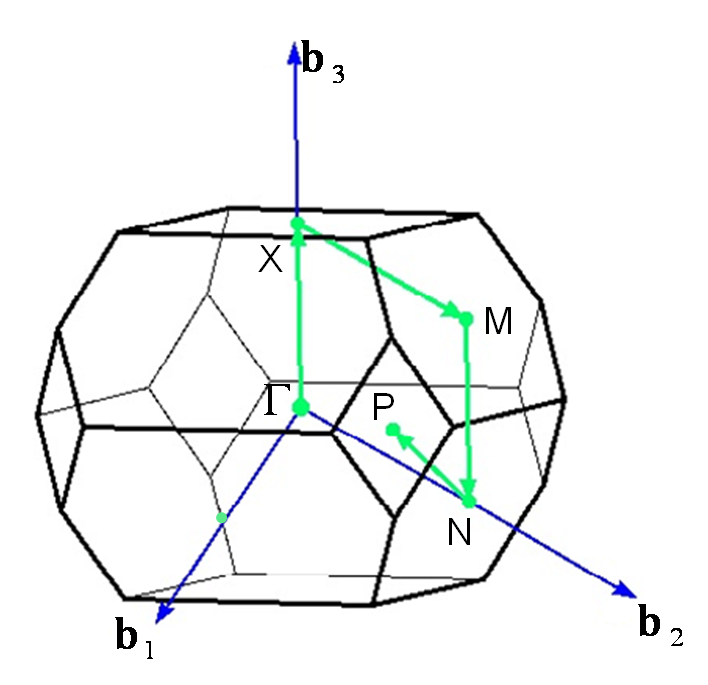
\includegraphics[height=50mm]{bz.eps}
\caption{The first Brillouin zone of CIGS.}
\label{bz}
\end{center}
\end{figure}

\noindent The first Brillouin zone (BZ) is the Wigner-Seitz primitive cell in reciprocal space, for example, the Fig. \ref{bz} is the first BZ of CIGS, where $\textbf{b}_1$, 
$\textbf{b}_2$ and $\textbf{b}_3$ are reciprocal lattice basis vectors. The following is the table about high symmetry points of the first BZ.


%\FloatBarrier
\vspace{10cm}


\begin{table}{}
\begin{center}
\begin{tabular}{|c|c|c|c|}
  \hline
  \multicolumn{4}{ | r |}{Points Coordinates($\textbf{b}_1$,$\textbf{b}_2$,$\textbf{b}_3$)} \\
  \hline
  $\Gamma$ & 0 & 0 & 0 \\
    \hline
   X & 0 & 0 & 1/2 \\
   \hline
   M & 0 & 1/2 & 1/2 \\
   \hline
   N & 0 & 1/2 & 0 \\
   \hline
   P & 1/2 & 1/2 & 1/2 \\
  \hline
\end{tabular}
\caption{\textit{High Symmetry Points of BZ for CIGS}.}
\end{center}
\end{table}



\section{Band structure and density-of-states}
\noindent In solid, there are huge amount of atoms which interact each other, the discrete of energy split into the huge number of state
 with small difference, those are defined as energy band, it is very important if one wants to know more about electrons or optical
 properties. The band structure of $\mathrm {CuIn_{0.5}Ga_{0.5}Se_{2}}$ is given as follows:

\begin{figure}[h]\label{bs}
\begin{center}
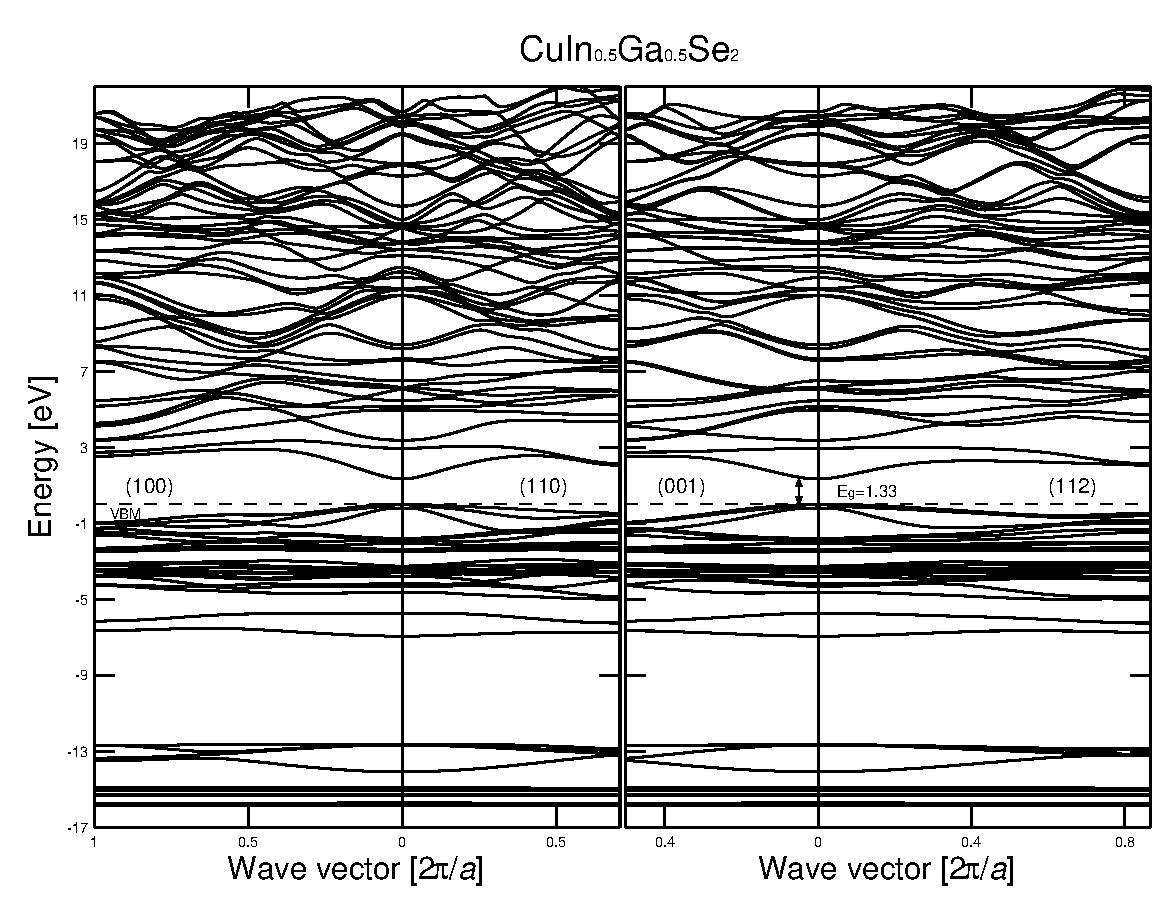
\includegraphics[height=90mm, width=110mm]{bandstr_theis.eps}
\caption{The band structure of CIGS.}
\end{center}
\end{figure}

\noindent The density of states (DOS) of a system is the number of states which could be occupied per interval of energy. The DOS of CIS is: 

\begin{figure}[H]
\begin{center}
%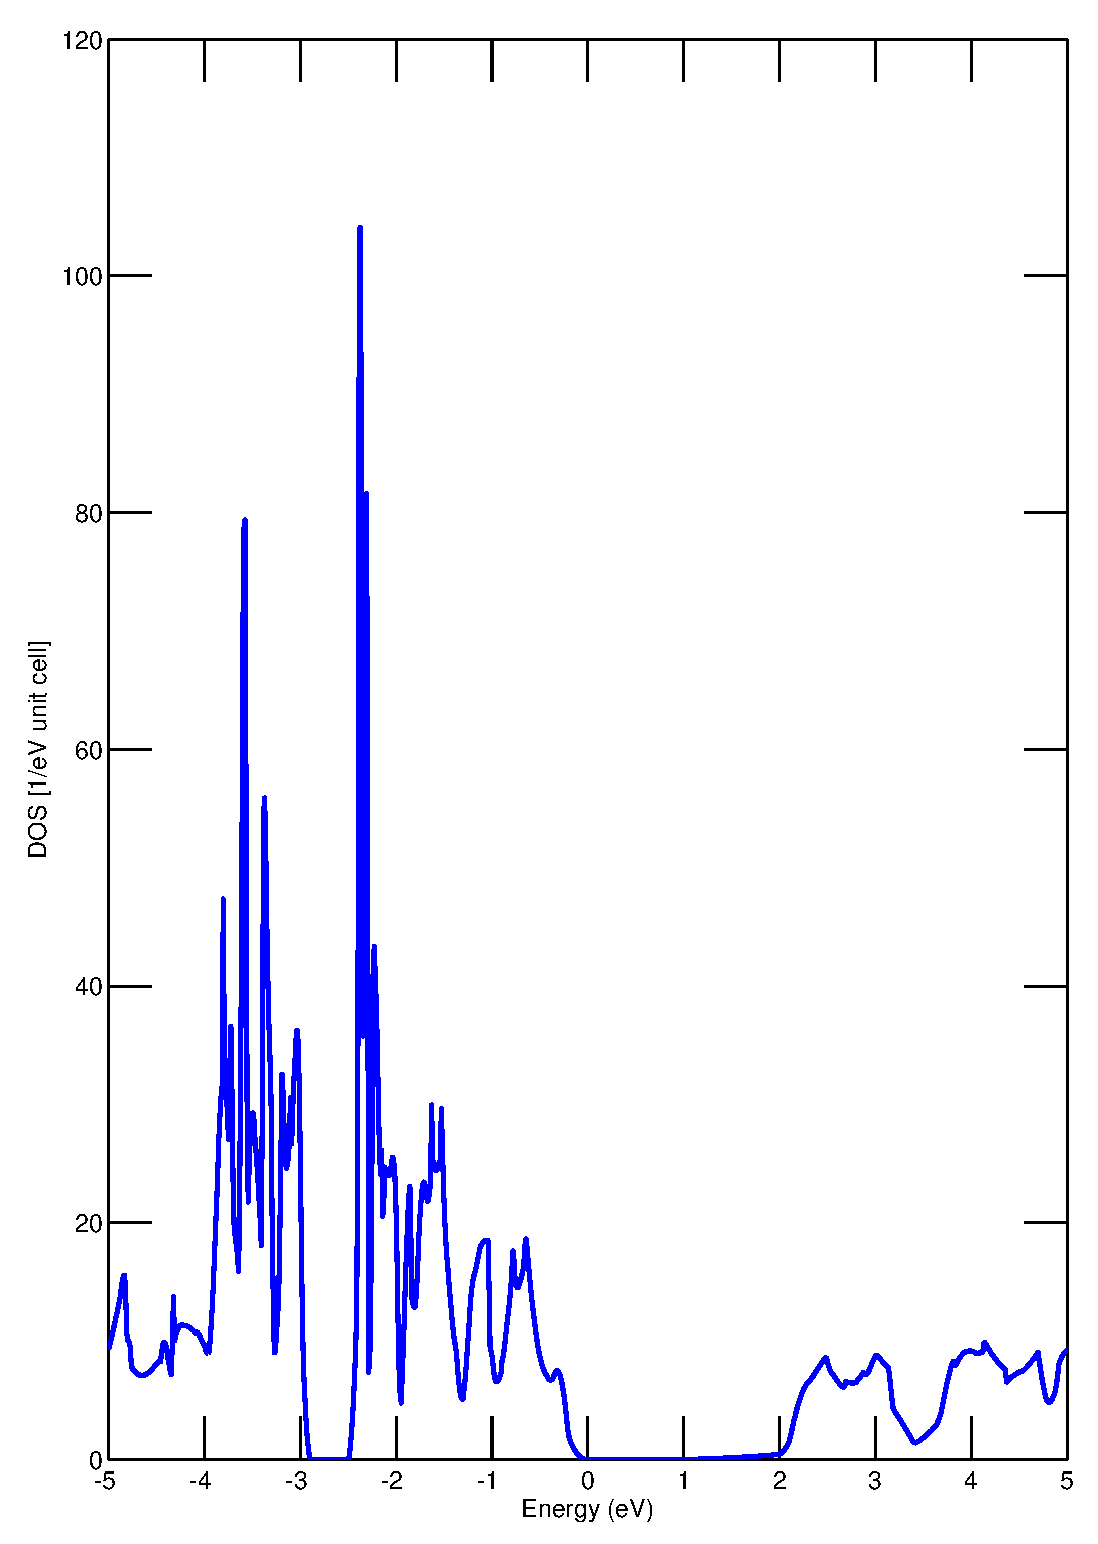
\includegraphics[scale=0.4]{totaldoscii.eps}
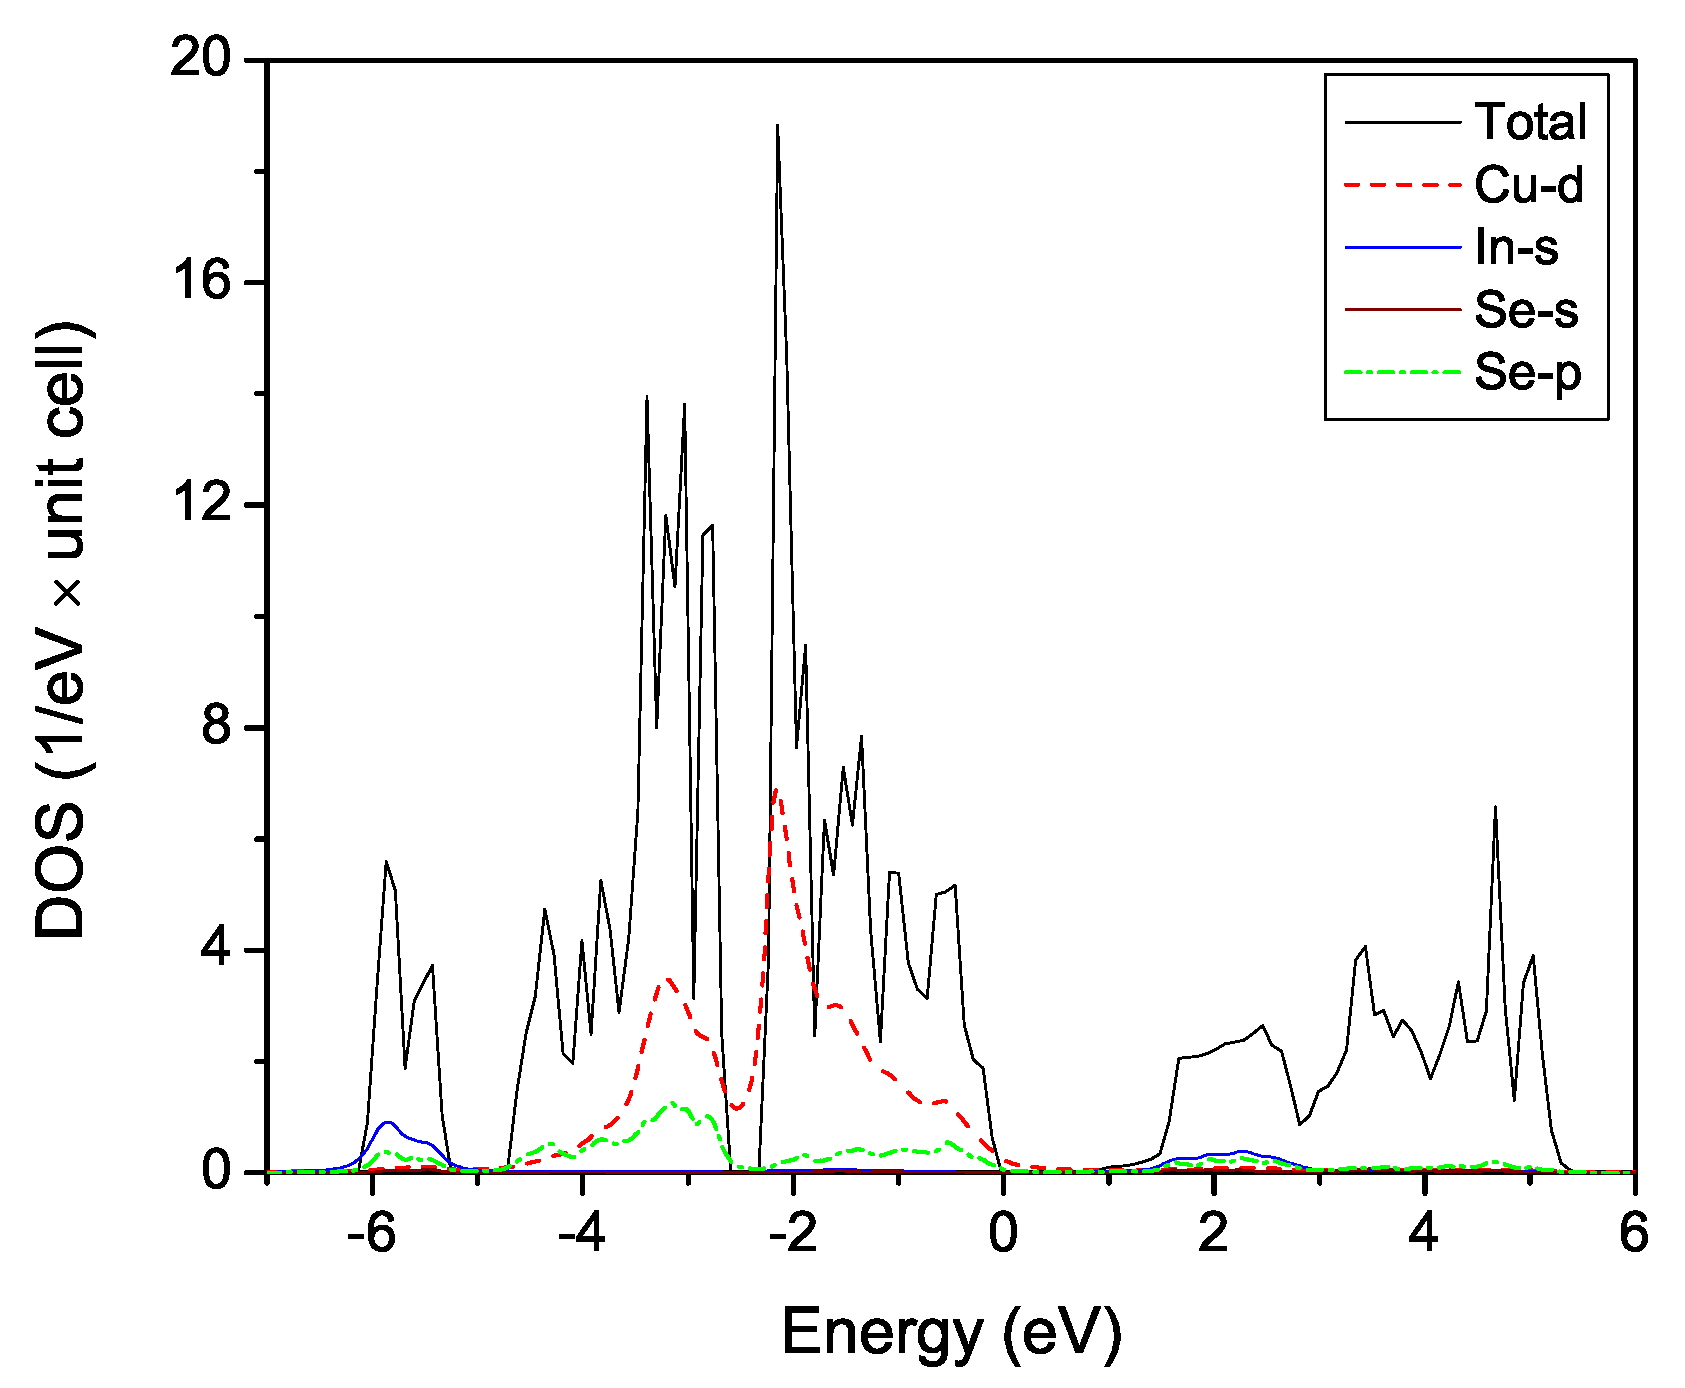
\includegraphics[height=90mm, width=110mm]{CuInSe2_PDOS.eps}
\caption{Density-of-states and of CIS.}
\label{doscis}
\end{center}
\end{figure}

where one can check from the Fig. \ref{doscis}, the band gap is around 1 eV. The Cu-d and Se-p are the main contribution in the range of 0 to -5 eV, 
moreover, the bonding strength between Cu-d and Se-p is stronger than In-s and Se-p.



\chapter{FP-LAPW method}
\section{Introduction}
\noindent So far, one already know how to solve the Kohn-Sham equation, however, there are still two more questions, what is the exact form of 
wavefunction and potential in the realistic calculation?  

\noindent One maybe naturally choose a set of plane waves as the wavefunction because of Bloch theory. There is a drawback about the plane wave 
when describing the atomic core region, because the wavefunction change dramatically, therefore one needs to choose more plane
waves to define it, which means it will take more time to calculate.

\noindent Slater re-consider the way to describe the wavefunction, he splits the unit cell into two regions, one is the sphere region which is
defined by the center of atom, but non-overlap each sphere, called muffin tin (MT) region, the remaining region is called interstitial 
(I) region (see Fig. \ref{ucuc}). An atomic-like function is defined as the wavefunction in MT region, this is reason why the method is called augmented plane wave (APW).
The dual representations of the wavefunction is reasonable, because the wave function approaching atomic core is somehow like inside atom, but far away the atomic core, the electron behaves like free electrons,
therefore plane wave is suitable (see Eq. (\ref{ap1})). However, the drawback of APW method is the wavefunction is dependent with the energy, which leads to the 
nonlinear eigenvalue problem (see Eq. (\ref{ap2})), in order to get the exact energy, the method has to decide repeatedly until certain condition is satisfied,
which is really time-consumming.
%%%%%%%%%%%%%%%%% figure of mf and ir

\noindent In order to find a way out, is it possible to let the wavefunction energy-independent? Andesen, Koelling and Arbman propose a way to describe that,
they notice that the taylor expansion of radial function (Eq. (\ref{ap3})), and then make use of it to linearize the APW method, thereby the method is called linearized augmented plane wave (LAPW)
method. However, the drawback is that this method does not describe the semicore state well, it is corrected by a method named linearized augmented plane wave plus local orbitals (LAPW+LO) which is proposed by Singh (Eq. (\ref{lap5})).
Sjöstedt, Nordström and Singh also give an efficient way to linearize Slater's APW method, named augmented plane wave plus local orbitals (APW+lo) (Eq. (\ref{lap6})).

%{\color{red}??????????????????? need to understant more about LAPW+LO and +lo ?????????????????????????} 


\section{Wavefunction}
\subsection{Augmented plane wave method}
\noindent Slater defines the wavefunction like the following equation:

%?????????????????????????????????????????????????????????????? comment here

\begin{equation}\label{ap1}
\phi^{APW}_{\textbf {k+G}} ({\textbf r})= 
\begin{cases} \frac {1}{\sqrt{\Omega}} e^{i({ \textbf {k+G}}) {\textbf r}} & \quad \mbox{if ${\textbf r} \in I $} 
\\
\sumg<\alpha>\sum\limits_{{\ell}m} f_{{\ell}{m}} (r_{\alpha},{\textbf {k+G}}, E) Y_{{\ell}m}(\widehat{{\textbf r}}_{\alpha})  & \quad \mbox{if $ {\textbf r} \in S_\alpha, $}\\ 
\end{cases}
\end{equation}





\noindent where $f_{{\ell}{m}} (r_{\alpha},\textbf{k+G} ,E) =  A _{{\ell}m}^{\alpha} ( \textbf {k+G}) u_{{\ell}}^{\alpha}(r_{\alpha}, E)$, and $A _{{\ell}m}^{\alpha} (\textbf {k+G}) $ is the expansion coefficients, and $u_{{\ell}}^{\alpha} (r_{\alpha}, E)$  is the radial function, which is dependent with energy $E$, and the
radial function could be decided by the following:


\begin{equation}\label{ap2}
-\frac{1}{r^2}  \frac{d}{dr} (r^2 \frac{du_{\ell}}{dr})+ \left(\frac{\ell(\ell+1)}{r^2}+V(r_{\alpha})\right)u_{\ell}(r_{\alpha}) = E u_{\ell}(r_{\alpha}),
\end{equation}


\noindent where $V(r_{\alpha})$ is the spherical potential.

%%%%%%%%%%%%%%%%%%%%%%  figure mt and interstial region

\noindent Because wavefunction has dual representations, one has to make sure the continousiny on the sphere, which is solved by matching each $\ell m$
of the dual representation.

\begin{figure}[h]
\begin{center}
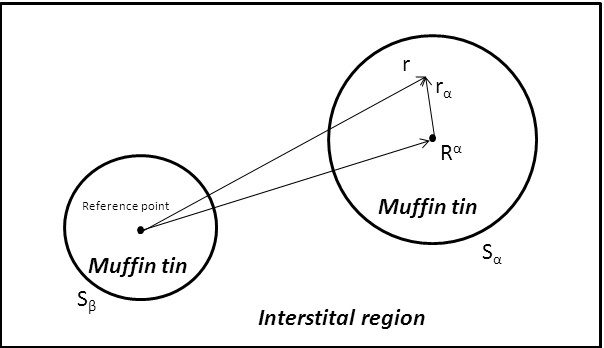
\includegraphics[scale=0.7]{Presentation1.png}
\caption{Partition of the unit cell.}
\label{ucuc}
\end{center}
\end{figure}


\noindent from the Fig. \ref{ucuc}, one will notice that the unit cell is divided into muffin-tin spheres ($\alpha$, $\beta$) and an
interstitial region (I), and ${\textbf r={\textbf R^{\alpha}}+{\textbf r_{\alpha}}}$ is guaranteed. so taking use of the Rayleigh expansion formula:

\begin{equation}
\expg<(\textbf {k+G})>= e^{i (\textbf {k+G}) \textbf{R}^{\alpha} } 4 \pi \sumlm<\ell><m> i^{\ell} \bessf< |\textbf{k+G}|> \sphfr<\ell{m}><r><> \sphfq<\ell{m}><\textbf{k+G}><*> .
\end{equation}
  
\noindent After matching those two representations, the following equation is satisfied for each ${\ell}m$:

\begin{equation}
A _{{\ell}m}^{\alpha} (\textbf {k+G})= \frac{ e^{i (\textbf {k+G}) \textbf{R}^{\alpha} } 4 \pi \sumlm<\ell><m> i^{\ell} \bessf< |\textbf{k+G}|> \sphfq<\ell{m}><\textbf{k+G}><*> }{\sqrt{\Omega} u_{{\ell}}^{\alpha}(r_{\alpha}, E)}.
\end{equation}

\noindent There are one main drawbacks about the APW method. The wavefuntion is energy dependent, which means that
 the code will search for the energy in order to calculate the exact energy. Therefore it 
is really time consuming. 

\subsection{Linearized augmented plane wave method}
\noindent In order to decouple the energy and wavefunction, Andesen, Koelling and Arbman find out a way to seperate them, they notice that the taylor expansion of the radial function
on certain energy, which can be expressed as follows:

\begin{equation}\label{ap3}
 u_{{\ell}}^{\alpha}(r_{\alpha}, E) = u_{{\ell}}^{\alpha}(r_{\alpha}, E_{\ell}) + (E-E_{\ell}) \dot{u}_{{\ell}}^{\alpha}(r_{\alpha}, E_{\ell}).
\end{equation}

\noindent So they re-define the wavefuntion in the following way:

%?????????????????????????????????????????????????????????????? comment here

\begin{equation}\label{lap4}
\phi^{LAPW}_\textbf{k+G} (\textbf{r})= 
\begin{cases} \frac {1}{\sqrt{\Omega}} e^{i(\textbf{k+G})\textbf{r}} & \quad \mbox{if $\textbf{r} \in I $}
\\
\sumg<\alpha>\sum\limits_{{\ell}m} f_{{\ell}{m}} (r_{\alpha},\textbf{k+G}, E_{\ell}) Y_{{\ell}m}(\hat{\textbf{r}}_{\alpha})  & \quad \mbox{if $\textbf{r} \in S_\alpha, $}\\ 
\end{cases}
\end{equation}


\noindent where $f_{{\ell}{m}} (r_{\alpha},\textbf{k+G} ,E_{\ell}) =  A _{{\ell}m}^{\alpha} (\textbf {k+G}) u_{{\ell}}^{\alpha}(r_{\alpha}, E_{\ell}) + B _{{\ell}m}^{\alpha} (\textbf {k+G}) \dot{u}_{{\ell}}^{\alpha}(r_{\alpha}, E_{\ell})$
. $A _{{\ell}m}^{\alpha} (\textbf {k+G})$ and $B _{{\ell}m}^{\alpha} (\textbf {k+G})$ are the expansion coefficients, and $\dot{u}_{{\ell}}^{\alpha}(r_{\alpha}, E_{\ell} )$ is the derivative of the radial function.

\noindent Here energy $E_{\ell}$  is considered as pre-calculated parameter, actually, it is chosen by the middle of  each $\ell$-character band, therefore this method is called linearized augmented plane wave (LAPW) method.

\noindent Apparently, LAPW method is more suitable in reality, because the wavefunction is decoupled with energy, but it has to match for two parameters,
fortunately, even though, it still use less time comparing with APW method. However, there is one drawbacks, what if energy difference is bigger enough in the same $ {\ell} $ charater, 
which the $E_{\ell}$ is correct? so this situation will cause big error, these states are called as semi-core state, for example, it exists in the actinides and the rare earths and so on.

\subsection{Linearized augmented plane wave method plus local orbitals}
Comparing with LAPW method, LAPW+LO method extend the basis set, and add smaller number of basis set, which has the following format:


\begin{equation}\label{lap5}
\phi^{LO}_\textbf{k+G} (\textbf{r})= 
\begin{cases} 0 & \quad \mbox{if $\textbf{r} \in I $}
\\
(A _{{\ell}m}^{\alpha}  u_{{\ell}}^{\alpha}(r_{\alpha}, E_{\ell}) + B _{{\ell}m}^{\alpha}  \dot{u}_{{\ell}}^{\alpha}(r_{\alpha}, E_{\ell}) + C _{{\ell}m}^{\alpha}  u_{{\ell}}^{\alpha}(r_{\alpha}, E^{\prime}_{\ell})){Y_{{\ell}m}(\hat{\textbf{r}}_{\alpha})} & \quad \mbox{if $\textbf{r} \in S_\alpha, $}\\ 
\end{cases}
\end{equation}
 
\noindent where $A _{{\ell}m}^{\alpha}$ and $B _{{\ell}m}^{\alpha}$ is matching value and derivate on the sphere boundary to zero, but not plane wave, and $E^{\prime}_{\ell}$ is
the chosen energy from semi-core state.

\subsection{Augmented plane wave method plus local orbitals}
\noindent Actually, there is one more method which will deal with the energy-denpendent case, which is called as augmented plane wave method plus local orbitals (APW+lo), the 
basis function has two kinds, one is similar with APW method, but only without the derivative terms, e.g., $f_{{\ell}{m}} (r_{\alpha},\textbf{k+G} ,E_{\ell}) =  A _{{\ell}m}^{\alpha} \textbf(k+G) u_{{\ell}}^{\alpha}(r_{\alpha}, E_{\ell})$.
Another basis function is:
\begin{equation}\label{lap6}
\phi^{lo}_\textbf{k+G} (\textbf{r})= 
\begin{cases} 0 & \quad \mbox{if $\textbf{r} \in I $}
\\
(A _{{\ell}m,lo}^{\alpha}  u_{{\ell}}^{\alpha}(r_{\alpha}, E_{\ell}) + B _{{\ell}m,lo}^{\alpha}  \dot{u}_{{\ell}}^{\alpha}(r_{\alpha}, E_{\ell}) ){Y_{{\ell}m}(\hat{\textbf{r}}_{\alpha})} & \quad \mbox{if $\textbf{r} \in S_\alpha. $}\\ 
\end{cases}
\end{equation}
 
\noindent The value of $A _{{\ell}m,lo}^{\alpha}$ and $B _{{\ell}m,lo}^{\alpha}$ are obtained by normalization and local orbital has zero value at the muffin tin boundary. This method can not deal with semicore states like LAPW+LO, 
however, it does increase the efficiency to linearize Slater's APW method.

\section{Effective potential}

The potential in the FP-LAPW method is also divided into two regions, the MT region and the interstital region.
\begin{equation*}\label{lap7}
V(\textbf{r})= 
\begin{cases} \sumg<{\textbf G}> V_{\textbf G} e^{i {\textbf G} {\textbf {r}  }} & \quad \mbox{if $\textbf{r} \in I $}
\\
 \sum\limits_{{\ell}m} V_{{\ell}m}^{\alpha} (r_{\alpha}) Y_{{\ell}m}(\hat{{\textbf r}}_{\alpha})  & \quad \mbox{if $\textbf{r} \in S_\alpha. $}\\ 
\end{cases}
\end{equation*}

\chapter{Dielectric function}
The dielectric function describes the optical property of a matrial, normally, it is written as $\varepsilon$, which has two parts, so $\varepsilon = \varepsilon_1
+ i \varepsilon_2$, where $\varepsilon_1$ denotes how much the material is polarized when an electric field is applied, and $\varepsilon_2$ is related with absorption of the material.

Here a summary of the basic derivation of dielectric function is presented using random-phase approximation (RPA).

Response to external electric field $E$ in the linear approximation:
\begin{equation}\label{df1}
D = \varepsilon E,
\end{equation}
where $D$ is electric displacement, and $E$ is the electric field.

After some derivations, the imaginary part of $\varepsilon$ is:
\begin{equation}\label{df2}
\varepsilon_2 = \frac{4 \pi e^2}{m^2\omega^2} \sum_{cv} \int d \textbf {k} <\Psi_{c{\textbf k}}|p^\alpha|\Psi_{v{\textbf k}}><\Psi_{v{\textbf k}}|p^\beta|\Psi_{c{\textbf k}}>\delta(\varepsilon_{c {\textbf k}}-\varepsilon_{c{\textbf k}}-\omega),
\end{equation}
where $c$ and $v$ run over the conduction bands and valence bands, for example, one can find the figure which is calculated using this equation in the paper of $??$.

The interband contribution of dielectric function is:
\begin{equation}\label{df2}
\varepsilon_2 = \frac{4 \pi e^2}{m^2\omega^2} \sum_{cv} \int d \textbf {k} <\Psi_{c{\textbf k}}|p^\alpha|\Psi_{v{\textbf k}}><\Psi_{v{\textbf k}}|p^\beta|\Psi_{c{\textbf k}}> (f(\varepsilon_{c \textbf k})-f(\varepsilon_{v \textbf k}))\delta(\varepsilon_{c {\textbf k}}-\varepsilon_{c{\textbf k}}-\omega),
\end{equation}
which is often calculated in the field that is related to optical property, for example, it is calculated in the paper of $??$, which is plotted in the figure of $??$ in 
that paper.

Here only some very basic equations are covered when it is related to calculate the dielectric function, if someone is interested in this toppic, one can find more detailed in the paper$??$.
\chapter{k $\cdot$ p method}

%%%%%%modify the sentences below


The band dispersion can be obtained exactly by using the $\bold k \cdot \bold p$ method in principle, the basic idea will be explained in the following text.

First, if the Schrödinger equation is defined as follows:

\begin{equation}\label{kpse}
\left\{ \frac {{\textbf p}^2} {2m} + V({\textbf r}) \right\} \wfbloch<n>< \bold k> = \ebloch<n><\bold k> \wfbloch<n><\bold k>,
\end{equation}

where ${\textbf p} = i \hbar \bigtriangledown $, and the Bloch theory shows:

\begin{equation}\label{1}
 \wfbloch<n><\bold k> = \expg<k> \ubloch<n><\bold k>,
\end{equation}

where $\wfbloch<n><\bold k>$ is the wave function on ${\textbf k}$ point for the {$\textit n$}th band, and $\expg<k>$ is plane wave, $\ubloch<n><\bold k>$ is a function which has the same a periodicity as the potential.

If substituting the Eq. \ref{1} to Eq. \ref{kpse}, it will end up the following equation:

\begin{equation}
 \{  \frac{{\textbf p}^2}{2m} + V({\textbf r }) + \frac{{\hbar^2 {\textbf k}^2}}{2m} + \frac{{\hbar \textbf {kp}}}{m} \} \ubloch<n><\bold  k>  =  \ebloch<n><\bold  k> \ubloch<n><\bold  k>.
\end{equation}

In the above equation, if $\textbf k = \textbf 0$, then the Hamiltonian turn out to be $H_0 = {\textbf p}^2 / {2m} + V({\textbf r })$. Here the first two terms are treated as unpertubation term, and pertubation term is seen as
$W={{\hbar^2 {\textbf k}^2}}/{2m} + {{\hbar \textbf {kp}}}/{m}$, the result will be as follows after treating the equation as pertubation.

\begin{equation}
 \ebloch<n><\bold k> = E_{n,\textbf 0} + \frac{{\hbar^2 {\textbf k}^2}}{2m} + \frac{ \hbar^2}{m^2} \suminj<i><j> \frac{|<\ubloch<n><\bold 0>|{\textbf {kp}}|\ubloch<n'><\bold  0>>|^2}{E_{n,\textbf 0} - E_{n',\textbf 0}}.
\end{equation}


Now let us suppose the wavefunction and energy are obtained by some procedures on $\bold k_0$ point, $\wfbloch<n><\bold  k_0>$ is the wavefunction and $\ebloch<n><\textbf  k_0>$ is the energy.
Another function is defined as follows:

\begin{equation}\label{2}
\chikp<n><\textbf k> = \expg<(\bold k-\bold {k_0})>  \wfbloch<n><\bold {k_0}>.
\end{equation}

The above function $\chikp<n><\textbf k> $ is expanded as wave function on ${ \textbf k}$ point, and then the wave function on the ${\textbf k}$ point is calculated by:
\begin{equation}\label{3}
\wfbloch<n><\bold k> =  {\sum\limits_{j}} C_{n,j}^{\bold k} \chikp<j><\bold k>. 
\end{equation}

From above equation, the wave function is known if the coefficient $C_{n,j}^{\bold k}$ is obtained, let us substitute the Eq. \ref{3} into Kohn-Sham Eq. \ref{kpse}.
Finally the following equation is obtained:

\begin{equation}\label{5}
{\sum\limits_{j}}  C_{n,j}^{\bold k} \left \{  \left [  \ebloch<j><\bold {k_0}> -  \ebloch<n><\bold k>  + \frac{{\hbar}^2}{2m} { (\bold {k}^2- \bold {k}_0^2)}    \right ] \delta_{j',j} + \frac{\hbar}{m} {(\bold {k}-\bold{k}_0)} {\textbf p_{j',j}} \right \} = 0,
\end{equation}

where ${\textbf p_{j',j}} = \langle \ubloch<j'><\bold {k_0}>| {\textbf p} | \ubloch<j><\bold {k_0}>  \rangle $.
 
We also can simpify the above equation in the following format:
\begin{equation}\label{6}
{\sum\limits_{j}} C_{n,j}^{\bold {k}} \left \{ H_{j',j}- \ebloch<n><\bold {k}> \delta_{j',j} \right \} =0,
\end{equation}

where
\begin{equation} \label{7}
H_{j',j} = \left [  \ebloch<j><\bold {k_0}>  + \frac{{\hbar}^2}{2m} { (\bold{k}^2-\bold{k}_0^2)}    \right ] \delta_{j',j} + \frac{\hbar}{m} {(\bold{k}-\bold{k}_0)} {\textbf p_{j',j}}.
\end{equation}

From the above equation, the coefficient $ C_{n,j}^{\bold k}$ is calculated.





\chapter{Summary}

\section{Parameterization of energy bands for $\cigs$}
In this work, the parameterization of energy bands (three uppermost valence bands and the lowest conduction band) is described in chalcopyrite $\cigs$ 
(x = 0, 0.5, and 1) alloys, with a more correct description of the energy dispersions, one can better analyze the electron and hole dynamics in the $\cigs$ alloys,
thereby better understand the electrical properties of these compounds. In order to demonstrate the anisotropic and non-parabolic of energy bands, some properties are investigated, such as effective 
electron and hole masses, constant energy surface and so on. To explain the importance of this parameterization, the DOS, Fermi energy and carrier
concentrations are analysed and compared with parabolic band dispersion.

All the detailed information can be obtained in the attached paper in this licentiate, so here only some figures not shown up in the attached paper are presented. 

First, the comparation between DOS from full band parameterization (fbp), parabolic band approximation (pba) and calculated using DFT is compared, the detailed can be seen from Fig. \ref{dos}:


\begin{figure}[H]
\begin{center}
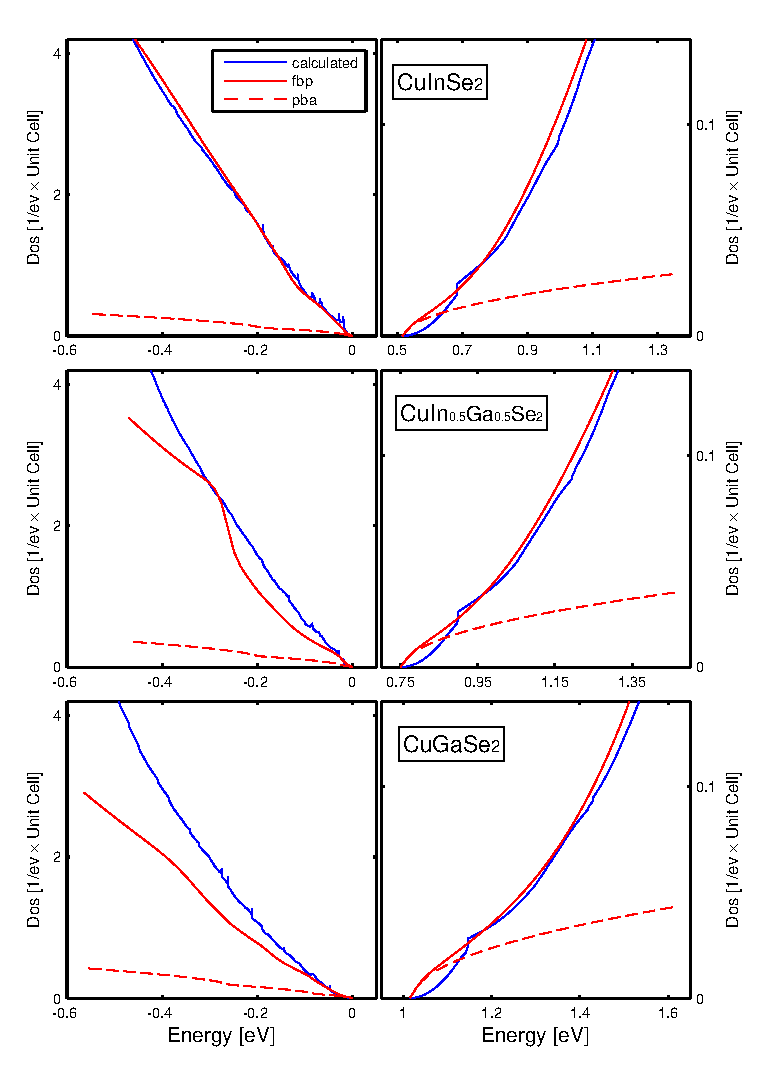
\includegraphics[scale=0.7]{figure5_clas.eps}
\caption{Density-of-states.}
\label{dos}
\end{center}
\end{figure}

From the Fig. \ref{dos}, one can notice that the DOS are more matched between fbp and calculated using DFT compared with pba, especitally, for the lowest conduction band since it is more isotropic compared
with valance bands.

In Fig. \ref{bbbbb}, the constant energy surfaces of ${\mathrm{ CuInSe_2}}$ and ${\mathrm{ CuGaSe_2}}$ are presented for the energies E = 1 meV 
and E = 200 meV, which demontrates that the energy bands are ellipsoidal in the vicinity of the $\Gamma$-point, but the VBs are very
non-parabolic and anisotropic at away from the the $\Gamma$-point. For example, the effective masses for the topmost VB for ${\mathrm{ CuInSe_2}}$  are anisotropic
($m^{\perp}_{v1}$ = 0.14$m_0$ and $m^{\parallel}_{v1}$ = 0.66$m_0$), so the constant energy surface is elllipsoidal in the vicinity of the  $\Gamma$-point. However,
far away $\Gamma$-point, the constant energy surface change dramatically. 
 

\begin{figure}[H]
\begin{center}$
\begin{array}{cc}
\includegraphics[scale=0.4]{ciithreedcii.eps} &
\includegraphics[scale=0.4]{cggthreedcgg.eps}
\end{array}$
\end{center}
\caption{Constant energy surface for ${\mathrm{ CuInSe_2}}$ and ${\mathrm{ CuGaSe_2}}$.}
\label{bbbbb}
\end{figure}


To summary in this work, we find out that the three uppermost VBs are strongly anisotropic and non-parabolic, however the lowest CB becomes non-parabolic for energies 50-100 meV
above the $\Gamma$-point band minimum. A constant DOS mass cannot accurately describe band filling of the VBs even at low hole concentrations. Instead, 
an energy dependent DOS mass is introduced that can be utilized to describe the carrier concentration and the Fermi energy using traditional equations for the DOS.
With the full description of the energy dispersion, the hole concentration is improved by a factor of 10–50 and the electron concentration is improved by a 
factor of 2–10 depending on quasi-Fermi energy. The transition from the freeze-out region to the extrinsic region occurs well below the room temperature for
uncompensated acceptor concentration below $~10^{17}$/$cm^3$, whereas for higher concentrations not all acceptors are ionized at T = 300 K. 

\section{Dielectric function spectra of $\mathrm {{Cu}{In}_{0.5}{Ga}_{0.5}{Se}_2}$}
%\section{Dielectric function spectra of $ {\textbf {Cu} \textbf  {In}_{0.5} \textbf  {Ga}_{0.5} \textbf {Se}_2}$ }
In this work, the $\varepsilon$ spectra of $\mathrm {CuIn_{0.5}Ga_{0.5}Se_2}$ which is calculated by FP-LAPW method is described and compared with experiment
result, then different contributions to $\varepsilon_2$ (Im$(\varepsilon)$) in terms of the transitions between the valence bands and the conduction bands are identified, at last, 
the $\textbf{k}$-dependence of the CPs along the main symmetry directions is analyzed. All the detailed description is presented in the attached paper.

Besides the figures presented in the attached paper, here there are two more figures shown in this section. The first one is the components of the $\varepsilon_2$ in terms of
xx, yy and zz directions, where the slightly difference amonge the components of xx, yy and zz is observed. Unfortunately, there are no experimental data to compare with $Im(\varepsilon_{xx}), Im(\varepsilon_{yy})$ and $Im(\varepsilon_{zz})$. Here,
$\varepsilon_2$ = ($Im(\varepsilon_{xx}) + Im(\varepsilon_{yy}) + Im(\varepsilon_{zz}) )/3$. 

\begin{figure}[H]
\begin{center}
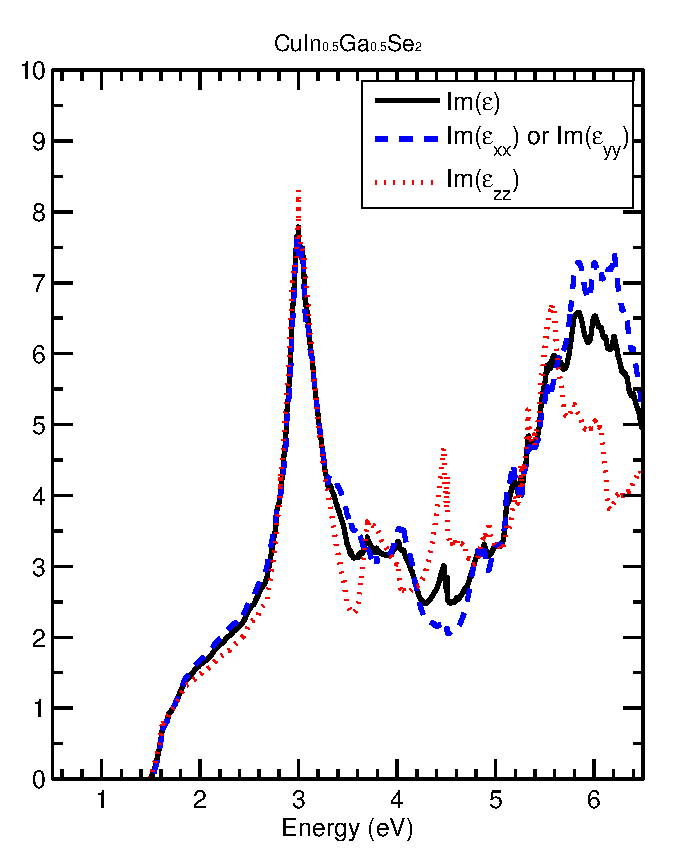
\includegraphics[scale=0.7]{thesis1.eps}
\end{center}
\caption{The $\varepsilon_2$ spectra for $\mathrm {CuIn_{0.5}Ga_{0.5}Se_2}$. }
\end{figure}

In Fig. \ref{ccccc} , the comparation of $\varepsilon_2$ between ${\mathrm{ CuInSe_2}}$ and $\mathrm {CuIn_{0.5}Ga_{0.5}Se_2}$  is shown, which demonstrates that both are quite similar in 
the calculated $\varepsilon_2$ spectrum and the CP features between ${\mathrm{ CuInSe_2}}$ and $\mathrm {CuIn_{0.5}Ga_{0.5}Se_2}$. However, the calculations from 
${\mathrm{ CuInSe_2}}$ show that the CPs of $E_2$ and $E_3$ occur 0.1 to 0.2 eV higher than the $E_1$ CP.

\begin{figure}[H]
\begin{center}
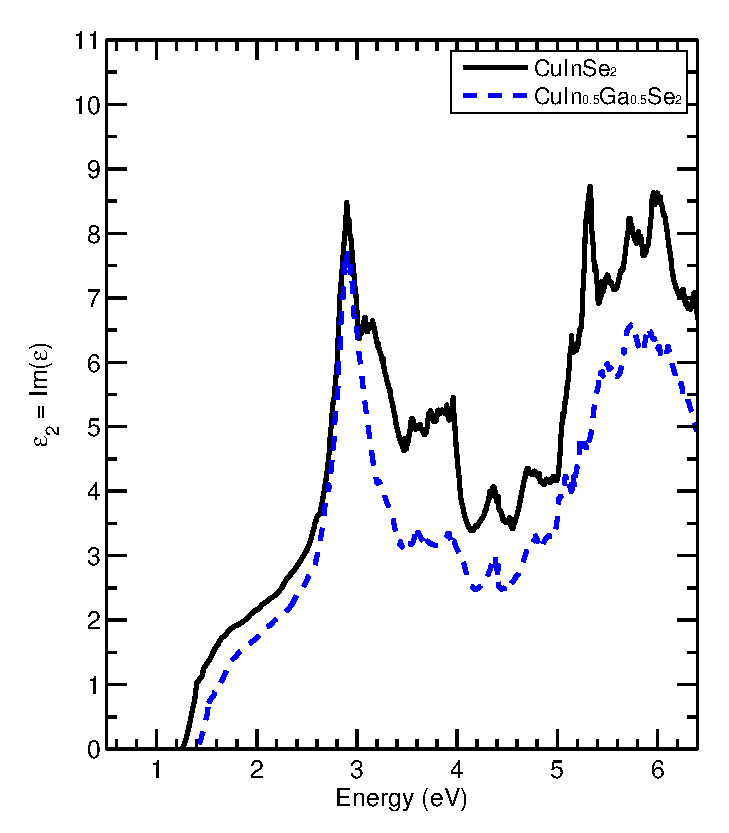
\includegraphics[scale=0.7]{thesis2.eps}
\end{center}
\caption{The $\varepsilon_2$ spectra for ${\mathrm{ CuInSe_2}}$ and $\mathrm {CuIn_{0.5}Ga_{0.5}Se_2}$. }
\label{ccccc}
\end{figure}

To summary in this work,the $\varepsilon$ spectra of $\mathrm {CuIn_{0.5}Ga_{0.5}Se_2}$ which is calculated by FP-LAPW method is described and compared with experiment
result. Electronic origins of the observed CP features
were discussed based on the results from FP-LAPW calculations of the electronic band structure for $\mathrm {CuIn_{0.5}Ga_{0.5}Se_2}$. The pairs of valence and conduction bands along 
the main symmetry directions of Brillouin zone were suggested for the major CP features observed in the $\varepsilon_2$ spectra.
\end{document}
